\subsection{Dataset}
Table \ref{tab:datasets} gives the current datasets we used for test. Datasets come from SNAP and KONECT.\\ 
web-Google dataset is Web graph from Google. \\
social-Youtube dataset is Youtube online social network. \\
roadMap-PA(CA/TX) dataset is Road network of Pennsylvania(California/Texas). \\
rating-Libimseti dataset is the network of ratings given by users of Libimseti.cz to other users. The network is unipartite, directed, and edges represent ratings on a scale from 1 to 10. 
\begin{table}[htbf]
\begin{center} 
\begin{tabular}{|l | c | c | c } \hline \hline 
Dataset & Type & Nodes & Edges \\ \hline
web-Google & Directed & 875,713 & 5,105,039 \\
social-Youtube & Undirected & 1,134,890 & 2,987,624 \\
roadMap-PA & Undirected & 1,088,092 & 3,083,796 \\
roadMap-CA & Undirected & 1,965,206 & 5,533,214 \\
roadMap-TX & Undirected & 1,379,917 & 3,843,320 \\
rating-Libimseti & Directed/Weighted & 220,970 & 17,359,346 \\ \hline
\end{tabular} 
\end{center} 
\caption{Test Datasets}
\label{tab:datasets} 
 \end{table}p{5cm}
 
 Besides that, we also define four typical test cases to indicate algorithm accuracy. \\
 Each test case has 5 nodes, as show in Figure \ref{fig:testcase}.
\begin{table}[htbf]
\begin{center} 
\begin{tabular}{|l | p{5cm} | } \hline \hline 
Case & Description \\ \hline
Star & one node serves as a hub, the rest of nodes form 1 degreee connect with hub and not connected to each other.\\
Chain & one node connected to a precedent and a follower node \\
Clique & every node has full connection to the rest of nodes in the group \\
Bi-partite& nodes are divided into two group, node in one group has full connection to the nodes at the other group,  but no connection to the nodes at the same group\\ \hline
\end{tabular} 
\end{center} 
\caption{Test Cases}
\label{tab:cases} 
 \end{table}

 \begin{figure}[htbf]
\begin{center}
\begin{tabular}{cc}
     % uncomment the next lines, and give the right ps files
     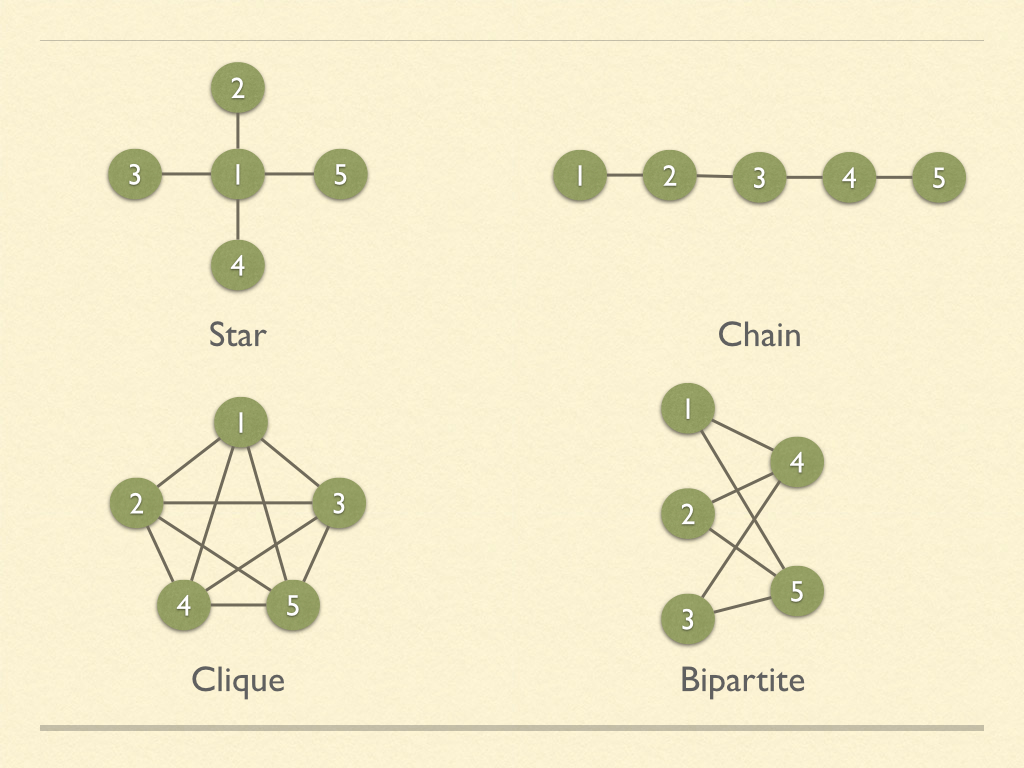
\includegraphics[width=0.6\textwidth]{FIG/testcase.jpg} \\
     %\psfig{figure=FIG/plot.ps,width=2in} \\
     % \psfig{figure=FIG/data.ps,width=2in} &
     % \psfig{figure=FIG/plot.ps,width=2in} \\
\end{tabular}
\caption{Test Case}
\label{fig:testcase}
\end{center}
\end{figure}

%%%%%%%%%%%%%%%%%%%%%%%%%%%%%%%%%%%%%%%%%%%%%%%%%%%%%%%%%%%

\subsection{Task 1: Degree Distribution}
\subsubsection{Accuracy Demonstration}
One way we use the veryify the result is to use the task case(which can be inferred manually). The reults we get from algorithm are as follows, which meet the values we expected.
\begin{verbatim}
Star:
 degree | count 
--------+-------
      1 |     4
      4 |     1

Chain:
 degree | count 
--------+-------
      1 |     2
      2 |     3

Clique:
 degree | count 
--------+-------
      4 |     5

Bipartite:
 degree | count 
--------+-------
      2 |     3
      3 |     2
\end{verbatim}

Another way is to check if the plot follows the power law in real dataset. We implemented the degree distribution method using SQL and performed the query on Facebook Social Circle dataset from SNAP
\footnote{SNAP: http://snap.stanford.edu/data/index.html}. The graph has 4039 vertices and 88234 edges. 

Figure \ref{fig:results} shows our results:
Figure \ref{fig:results}(a) gives a scatter-plot of the in-degree distribution on a log-log scale for the Facebook graph dataset.
Figure \ref{fig:results}(b) shows the out-degree distirbution.
X axis indicates the in-degree and y axis indicates the number of vertices which have the same in-degree or out-degree. 
According to the figures, We can easily observe the Power Law(heavy-tailed degree distribution) pattern.

\begin{figure}[htbf]
\begin{center}
\begin{tabular}{cc}
     % uncomment the next lines, and give the right ps files
     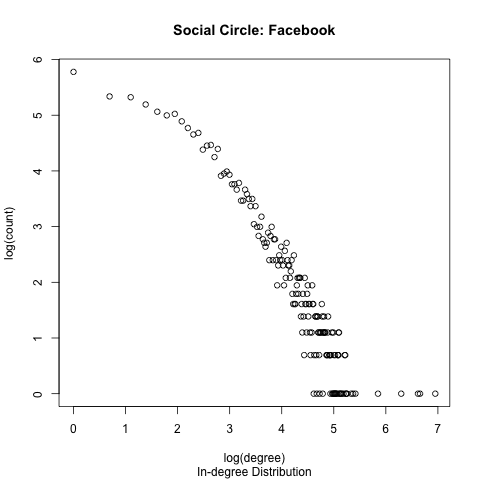
\includegraphics[width=0.5\textwidth]{FIG/in_degree.png} &
     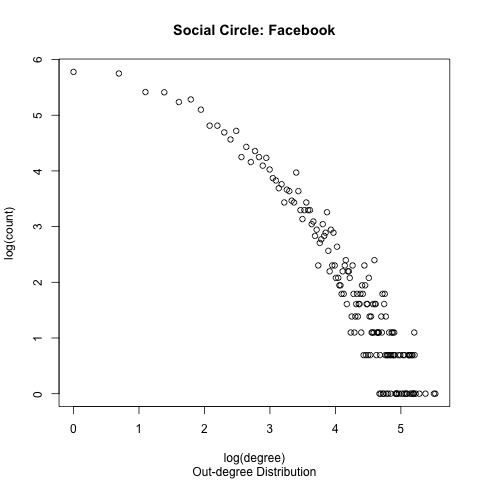
\includegraphics[width=0.5\textwidth]{FIG/out_degree.png} \\
     %\psfig{figure=FIG/plot.ps,width=2in} \\
     % \psfig{figure=FIG/data.ps,width=2in} &
     % \psfig{figure=FIG/plot.ps,width=2in} \\
    (a) & (b) 
\end{tabular}
\caption{The in-degree distribution plot(a) and out-degree distribution plot (b) on a log-log scale for Facebook graph dataset}
\label{fig:results}
\end{center}
\end{figure}

\subsubsection{Variety  Demonstration}
We perform the test on five 1M node datasets: web-Google(directed), social-Youtube, roadMap-PA, roadMap-CA, and roadMap-TX. Figure \ref{fig:results1} shows the result.\\
From the result we can find the heavy-tailed power law distribution from every figure, which shows that real dataset are very skewed distributed.\\
What we can also find is the difference between social network/web graph and road network graph. Road network turns out to have very small number in terms of degree. This actually make sense because degree represent the number of direct neighbours. While a webpage can link to hundreds of other webpages, or a person could have millions of follower on social network, a road in real life actually connect to only a few of roads.
\begin{figure}
    \centering
    \begin{subfigure}[htbp]{0.9\textwidth}
            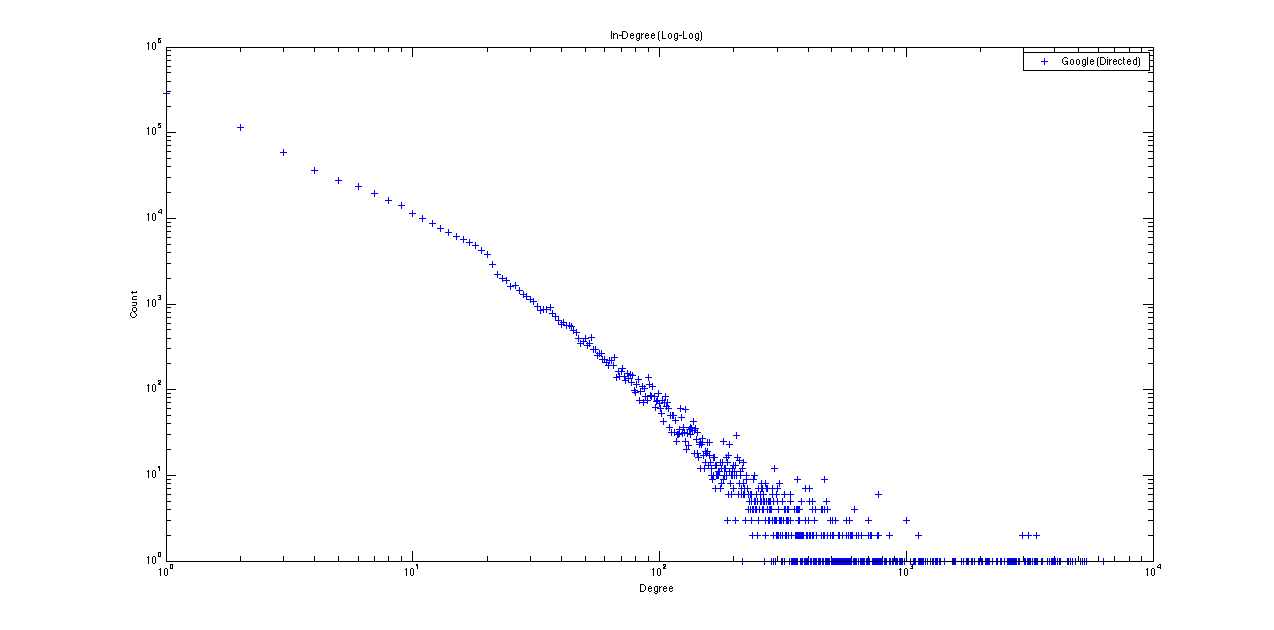
\includegraphics[width=\textwidth]{FIG/dd-google-in.png}
            \caption{Google in-Degree}
            \label{fig:dd-google-in}
    \end{subfigure}
    ~ %add desired spacing between images, e. g. ~, \quad, \qquad etc.
      %(or a blank line to force the subfigure onto a new line)
    \begin{subfigure}[htbp]{0.9\textwidth}
            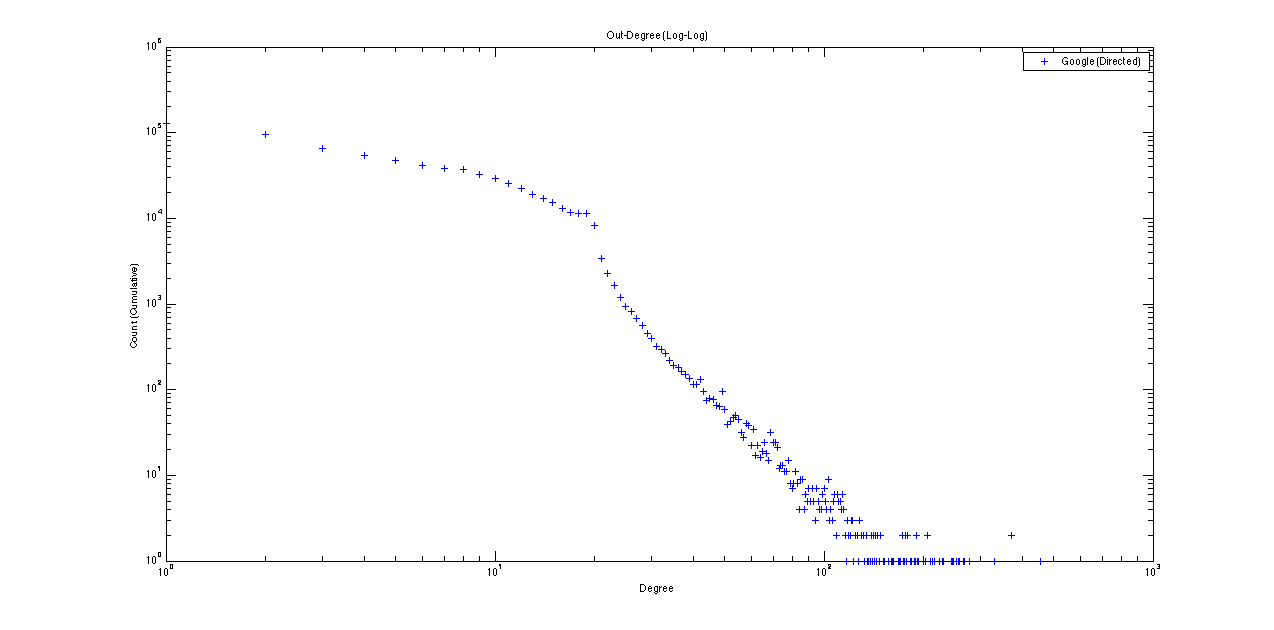
\includegraphics[width=\textwidth]{FIG/dd-google-out.png}
            \caption{Google out-Degree}
            \label{fig:dd-google-out}
    \end{subfigure}
    ~ %add desired spacing between images, e. g. ~, \quad, \qquad etc.
      %(or a blank line to force the subfigure onto a new line)
    \begin{subfigure}[htbp]{0.9\textwidth}
            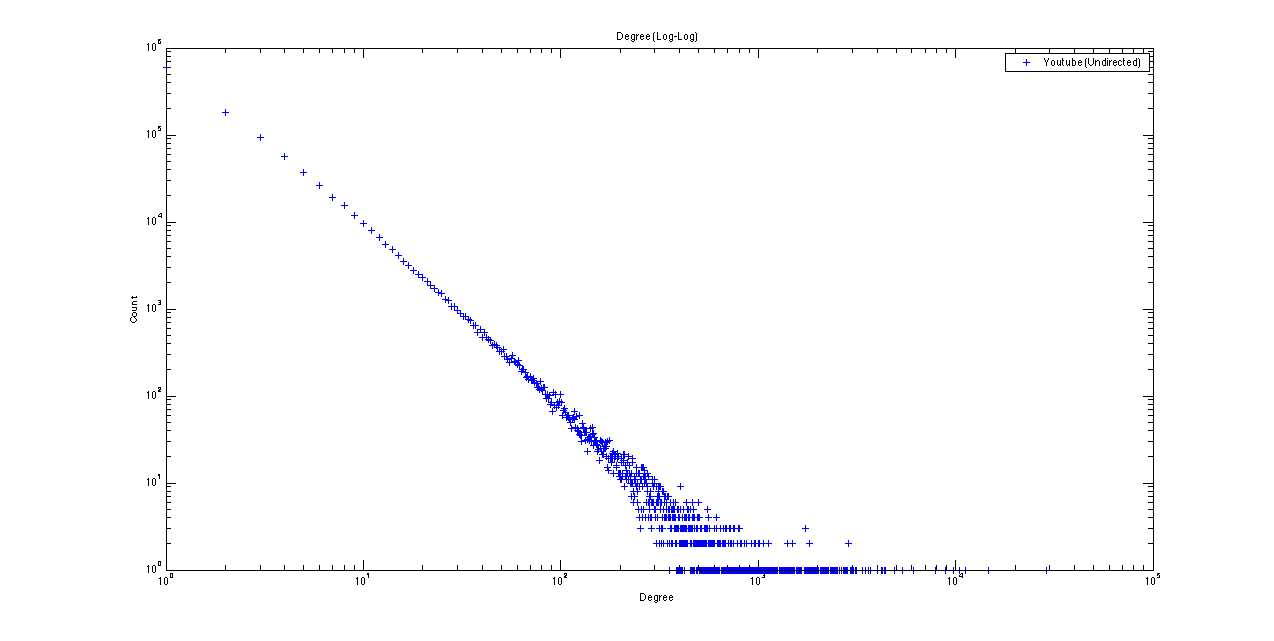
\includegraphics[width=\textwidth]{FIG/dd-youtube.png}
            \caption{Youtube}
            \label{fig:dd-youtube}
    \end{subfigure}
\end{figure} 

\addtocounter{figure}{-1}

\begin{figure} 
    \addtocounter{figure}{1}
    \centering 
        % ~ %add desired spacing between images, e. g. ~, \quad, \qquad etc.
          %(or a blank line to force the subfigure onto a new line)
        \begin{subfigure}[htbp]{0.9\textwidth}
                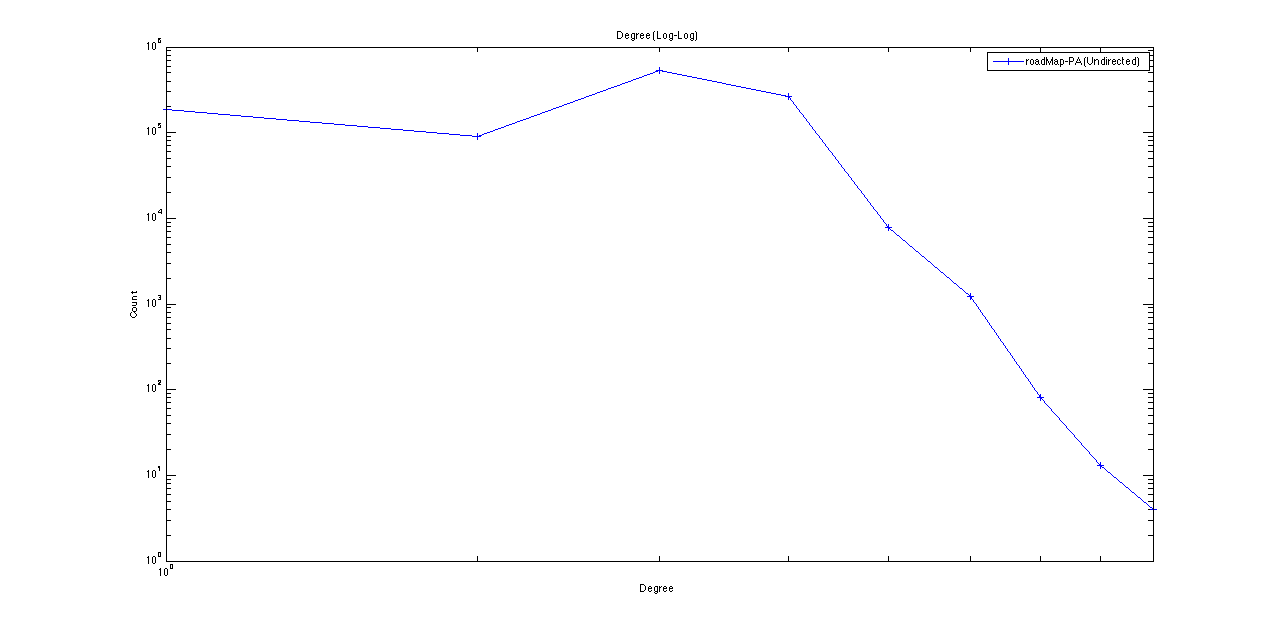
\includegraphics[width=\textwidth]{FIG/dd-pa.png}
                \caption{roadMap-PA}
                \label{fig:dd-pa}
        \end{subfigure}
        ~ %add desired spacing between images, e. g. ~, \quad, \qquad etc.
          %(or a blank line to force the subfigure onto a new line)
        \begin{subfigure}[htbp]{0.9\textwidth}
                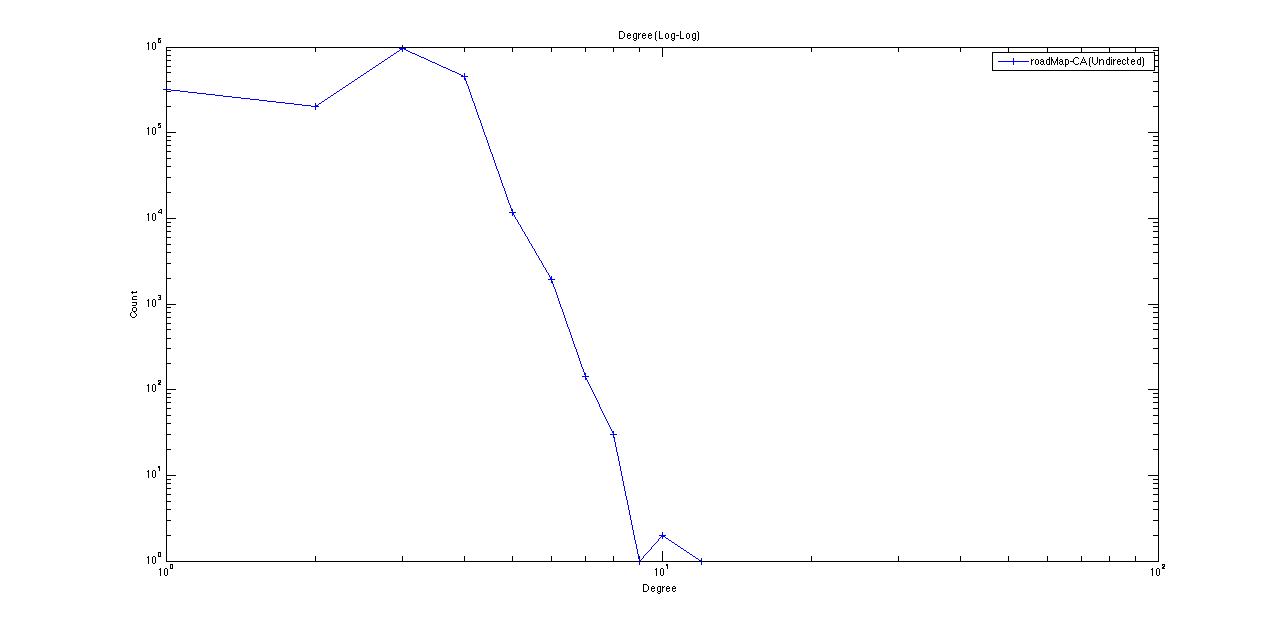
\includegraphics[width=\textwidth]{FIG/dd-ca.png}
                \caption{roadMap-CA}
                \label{fig:dd-ca}
        \end{subfigure}
        ~ %add desired spacing between images, e. g. ~, \quad, \qquad etc.
          %(or a blank line to force the subfigure onto a new line)
        \begin{subfigure}[htbp]{0.9\textwidth}
                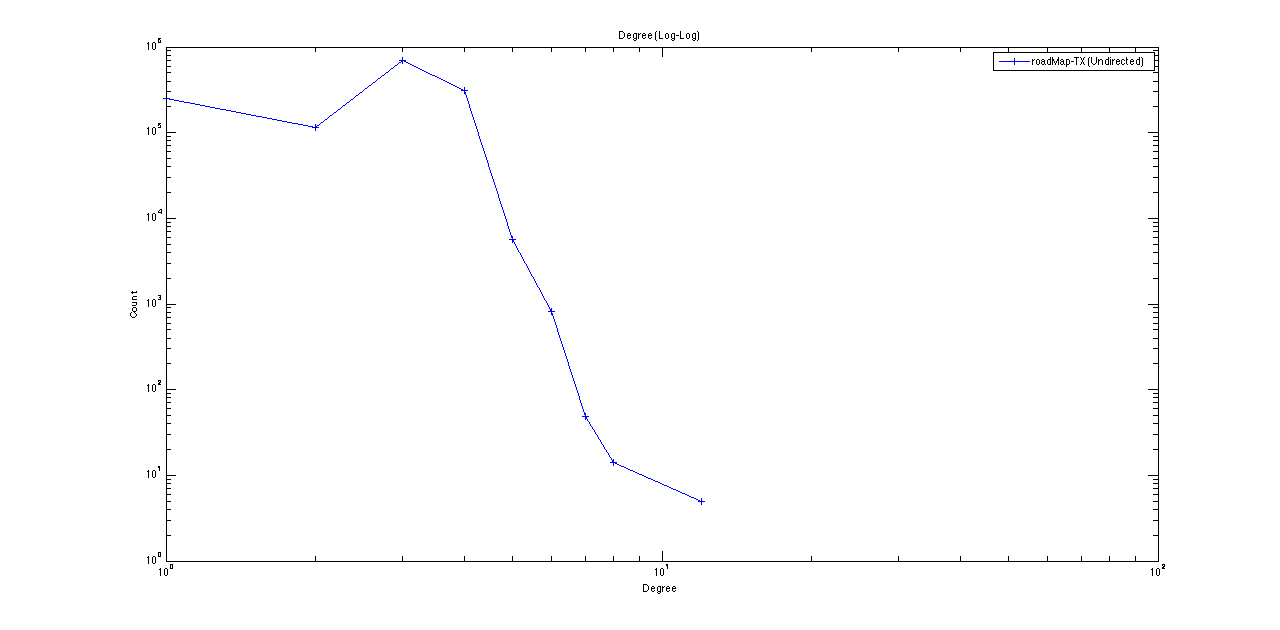
\includegraphics[width=\textwidth]{FIG/dd-tx.png}
                \caption{roadMap-TX}
                \label{fig:dd-tx}
        \end{subfigure}
        \caption{Degree Distribution}
        \label{fig:results1}
\end{figure}

%%%%%%%%%%%%%%%%%%%%%%%%%%%%%%%%%%%%%%%%%%%%%%%%%%%%%%%%%%%%%%%%%%%%%%%%%%%%%%%%%%%%%%%%%

\subsection{Task 2: Page Rank}
\subsubsection{Accuracy Demonstration}
We can also use the test case to tell if the PageRank computed by the algorithm is accurate. Consider the directed version of Star test case, where the hub(node 1) is pointed from every other nodes(node 2,3,4,5).\\
The result we get actually reflect the graph structure, where the hub has a higher rank and the rest of nodes share the same lower rank.
\begin{verbatim}
 v_row |       v_val        
-------+--------------------
     1 |                0.2
     2 | 0.0551136364533462
     3 | 0.0551136364533462
     4 | 0.0551136364533462
     5 | 0.0551136364533462
\end{verbatim}
Another thing we need to verify is the convergence of PageRank. Here we give the number of rank in iteration 10 and iteration 100. The result indicates that the rank computed by our algorithm coverges.
\begin{verbatim}
Iteration 10:
 v_row |       v_val        
-------+--------------------
     1 |                0.2
     2 | 0.0551136364533462
     3 | 0.0551136364533462
     4 | 0.0551136364533462
     5 | 0.0551136364533462
Iteration 100:
 v_row |       v_val        
-------+--------------------
     1 |                0.2
     2 | 0.0551136363636364
     3 | 0.0551136363636364
     4 | 0.0551136363636364
     5 | 0.0551136363636364
\end{verbatim}


\subsubsection{Variety Demonstration}
We perform the test on five 1M node datasets: web-Google(directed), social-Youtube, roadMap-PA, roadMap-CA, and roadMap-TX. Figure \ref{fig:results2} shows the result.\\
Notice that we are using cumulative count here in terms of the y-axis. That is, while x is the PageRank of a specific point, y is the number of points with greater PageRank value than that point.\\
From the figure we can figure out that both Youtube and Google graph follow the Power Law distribution of PageRank, which is pointed out in the paper \cite{Brin:1998:ALH:297810.297827}, while the roadMap datasets behave a little differently: only the latter part of the plot looks like power low distribution.

\begin{figure}
    \centering
    \begin{subfigure}[htbp]{0.9\textwidth}
            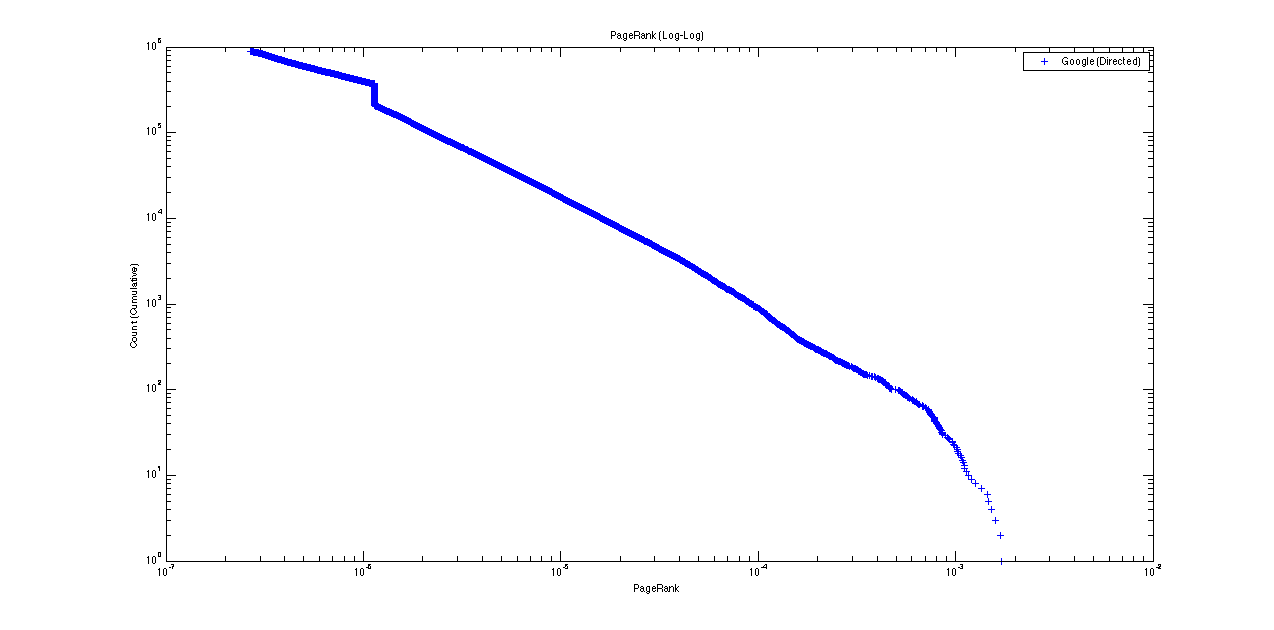
\includegraphics[width=\textwidth]{FIG/pr-google.png}
            \caption{Google}
            \label{fig:pr-google}
    \end{subfigure}
    ~ %add desired spacing between images, e. g. ~, \quad, \qquad etc.
      %(or a blank line to force the subfigure onto a new line)
    \begin{subfigure}[htbp]{0.9\textwidth}
            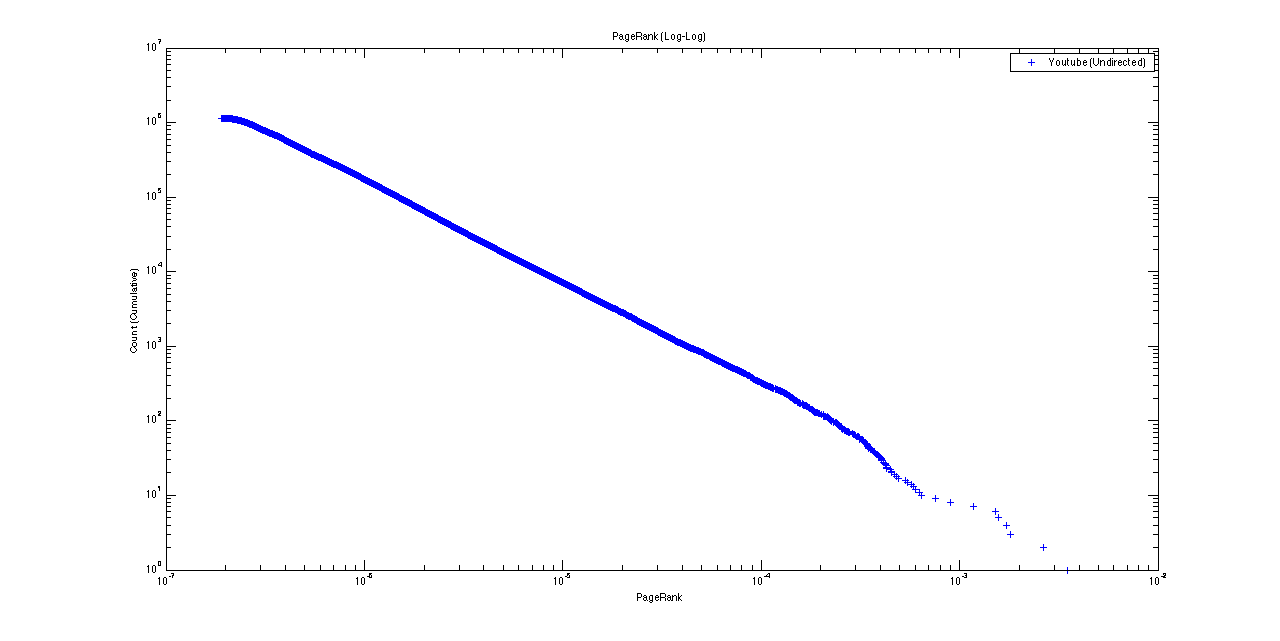
\includegraphics[width=\textwidth]{FIG/pr-youtube.png}
            \caption{Youtube}
            \label{fig:pr-youtube}
    \end{subfigure}
\end{figure} 

\addtocounter{figure}{-1}

\begin{figure} 
    \addtocounter{figure}{1}
    \centering 
        % ~ %add desired spacing between images, e. g. ~, \quad, \qquad etc.
          %(or a blank line to force the subfigure onto a new line)
        \begin{subfigure}[htbp]{0.9\textwidth}
                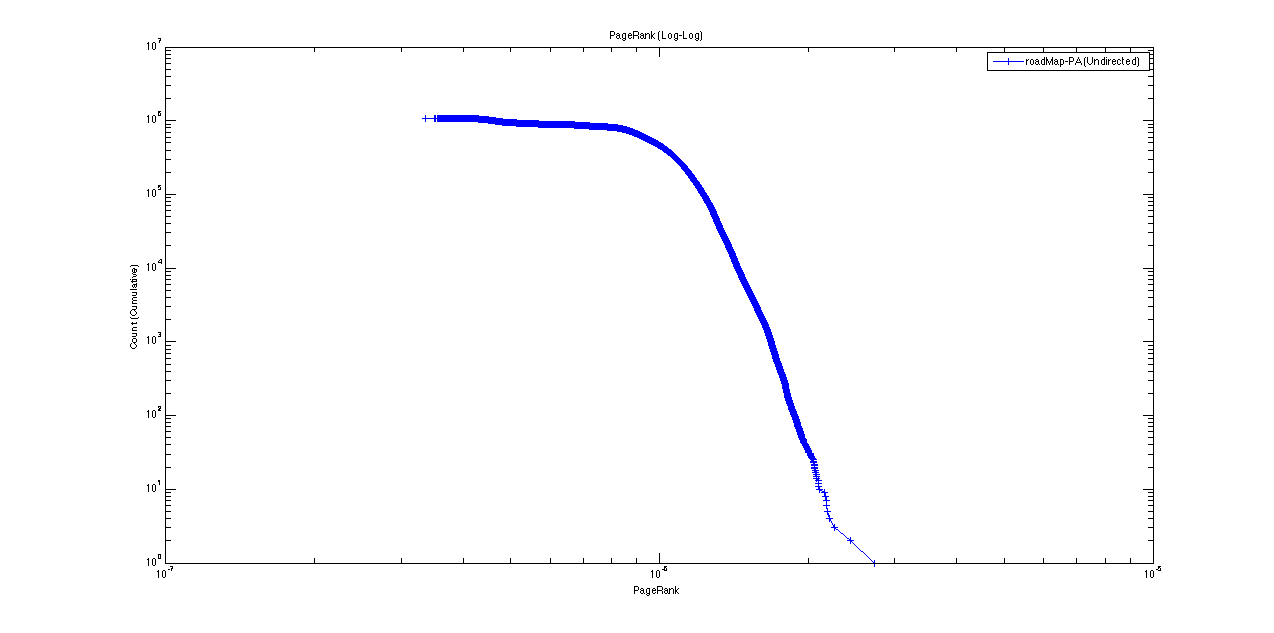
\includegraphics[width=\textwidth]{FIG/pr-pa.png}
                \caption{roadMap-PA}
                \label{fig:pr-pa}
        \end{subfigure}
        ~ %add desired spacing between images, e. g. ~, \quad, \qquad etc.
          %(or a blank line to force the subfigure onto a new line)
        \begin{subfigure}[htbp]{0.9\textwidth}
                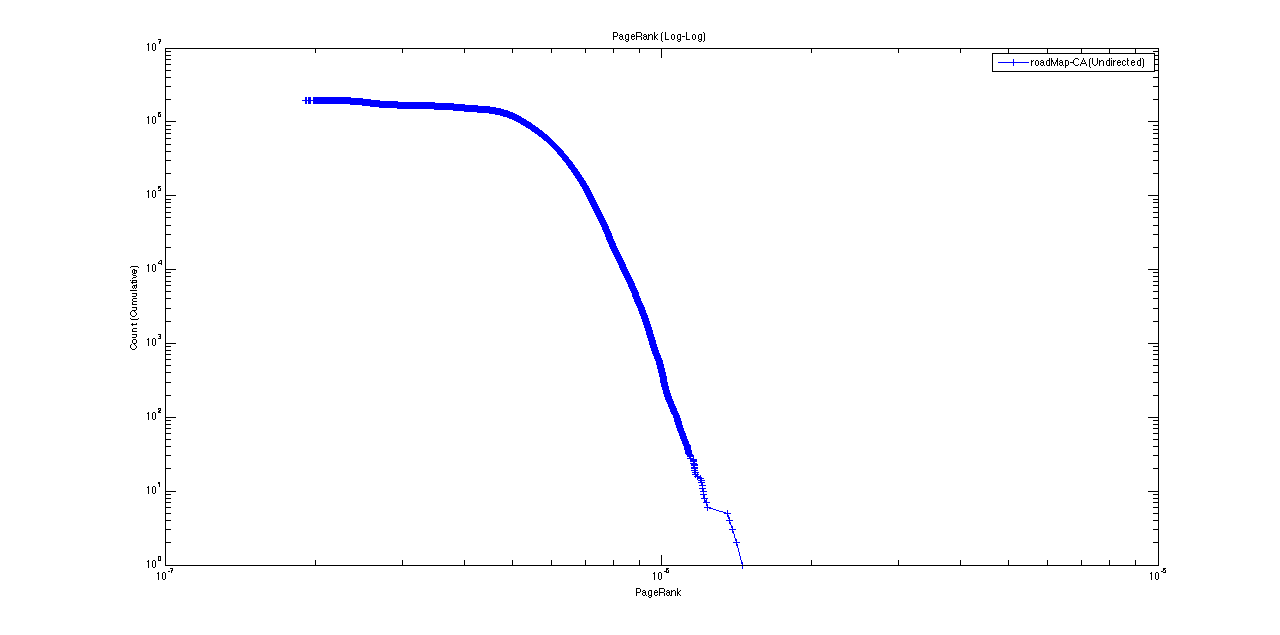
\includegraphics[width=\textwidth]{FIG/pr-ca.png}
                \caption{roadMap-CA}
                \label{fig:pr-ca}
        \end{subfigure}
        ~ %add desired spacing between images, e. g. ~, \quad, \qquad etc.
          %(or a blank line to force the subfigure onto a new line)
        \begin{subfigure}[htbp]{0.9\textwidth}
                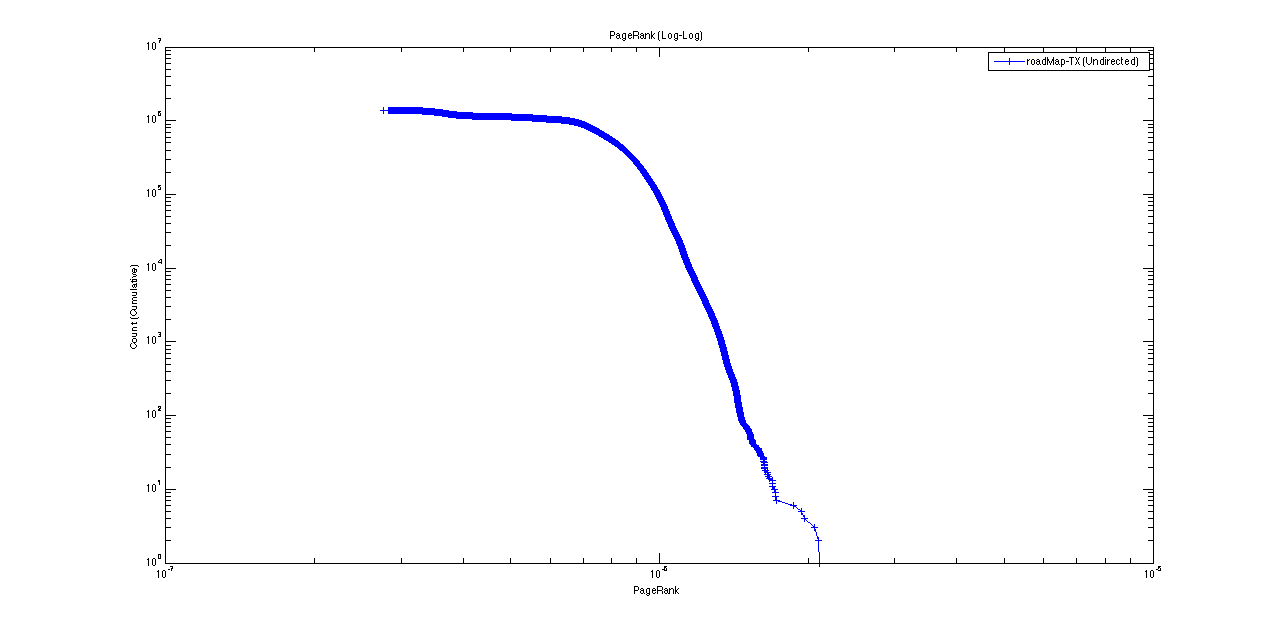
\includegraphics[width=\textwidth]{FIG/pr-tx.png}
                \caption{roadMap-TX}
                \label{fig:pr-tx}
        \end{subfigure}
        \caption{PageRank Distribution}
        \label{fig:results2}
\end{figure}

% We are in the progress of implementing Page Rank. We performed the first version of our code on Adjective-noun dataset from KONECT
% \footnote{KONECT: http://konect.uni-koblenz.de/networks/}. The graph has 86 vertices and 108 edges. 

% Figure \ref{fig:results2} shows our results. 
% X-axis indicates the number of nodes while y-axis gives the page rank.
% As can be seen in the graph, the nodes are normally distributed. Because this is a undirected graph, the page rank reveals the degree of each node.

% \begin{figure}[htbf]
% \begin{center}
% \begin{tabular}{cc}
%      % uncomment the next lines, and give the right ps files
%      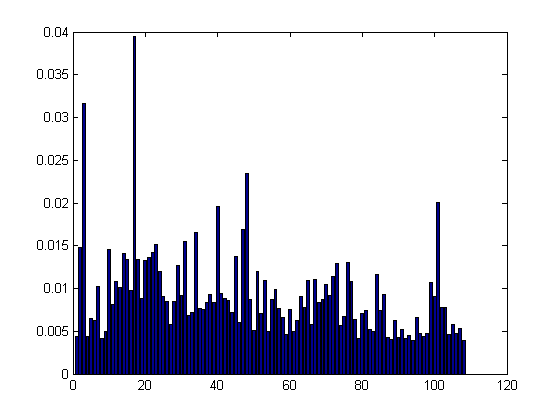
\includegraphics[width=0.6\textwidth]{FIG/task2.png} \\
%      %\psfig{figure=FIG/plot.ps,width=2in} \\
%      % \psfig{figure=FIG/data.ps,width=2in} &
%      % \psfig{figure=FIG/plot.ps,width=2in} \\
% \end{tabular}
% \caption{The Page-Rank plot for Adjective-noun dataset}
% \label{fig:results2}
% \end{center}
% \end{figure}

%%%%%%%%%%%%%%%%%%%%%%%%%%%%%%%%%%%%%%%%%%%%%%%%%%%%%%%%%%%%%%%%%%%%%%%%%%%%%%%%%%%%%%%%%

\subsection{Task 3: Connected Components}
\subsubsection{Accuracy Demonstration}
We use the test case to verify if the connected components computed by the algorithm is accurate. \\
Here we combines 4 test cases into one graph: node 1-5 belongs to Star graph; node 11-15 belongs to chain graph; node 21-25 belongs to clique graph; node 31-35 belongs to bipartite.\\
As for result, we expect to see four component each with size of 5. And the result are given as follows, which satisfies our expectation.\\
\begin{verbatim}
 node | comp 
------+------
    1 |    1
    2 |    1
    3 |    1
    4 |    1
    5 |    1
   11 |   11
   12 |   11
   13 |   11
   14 |   11
   15 |   11
   21 |   21
   22 |   21
   23 |   21
   24 |   21
   25 |   21
   31 |   31
   32 |   31
   33 |   31
   34 |   31
   35 |   31
\end{verbatim}
As for the convergence test, we modify the test case above by connecting four sub graph together, i.e. add three edges: 1-11, 11-21, 21-31. From the result given, we can tell that it costs five round for the algorithm to converge and the whole graph is formed in to a giant connected component, which is exactly what we expect.

\begin{verbatim}
 node | comp 
------+------
    1 |    1
    2 |    1
    3 |    1
    4 |    1
    5 |    1
   11 |    1
   12 |    1
   13 |    1
   14 |    1
   15 |    1
   21 |    1
   22 |    1
   23 |    1
   24 |    1
   25 |    1
   31 |    1
   32 |    1
   33 |    1
   34 |    1
   35 |    1
(20 rows)

Time: 0.813 ms
 round | gcc_count 
-------+-----------
     1 |         6
     2 |         8
     3 |        14
     4 |        17
     5 |        20
\end{verbatim}

\subsubsection{Variety Demonstration}
We perform the test on five 1M node datasets: web-Google(directed), social-Youtube, roadMap-PA, roadMap-CA, and roadMap-TX. Figure \ref{fig:results3} shows the result of convergence.\\
From the figure, we can see that Google and Youtube graph converge in around 10 iterations. However, roadMap-PA graph did not reach to convergen after the maximum iteration(which is set to 256). \\
The big difference from social network/web graph and roadnet graph still exists here. Although it takes only a few iteration for the network/graph to converge, the road graphs take far more rounds. The situation makes good sense because it exactly reflect the effect of small diameter/small world/six degree of seperation in terms of social network and web graph. \\
Meanwhile, the common sense confirms us that road networks are supposed to have long chain and large radius/diameter, which means far more iterations for the connected components to converge.\\
\begin{figure}
    \centering
    \begin{subfigure}[htbp]{0.8\textwidth}
            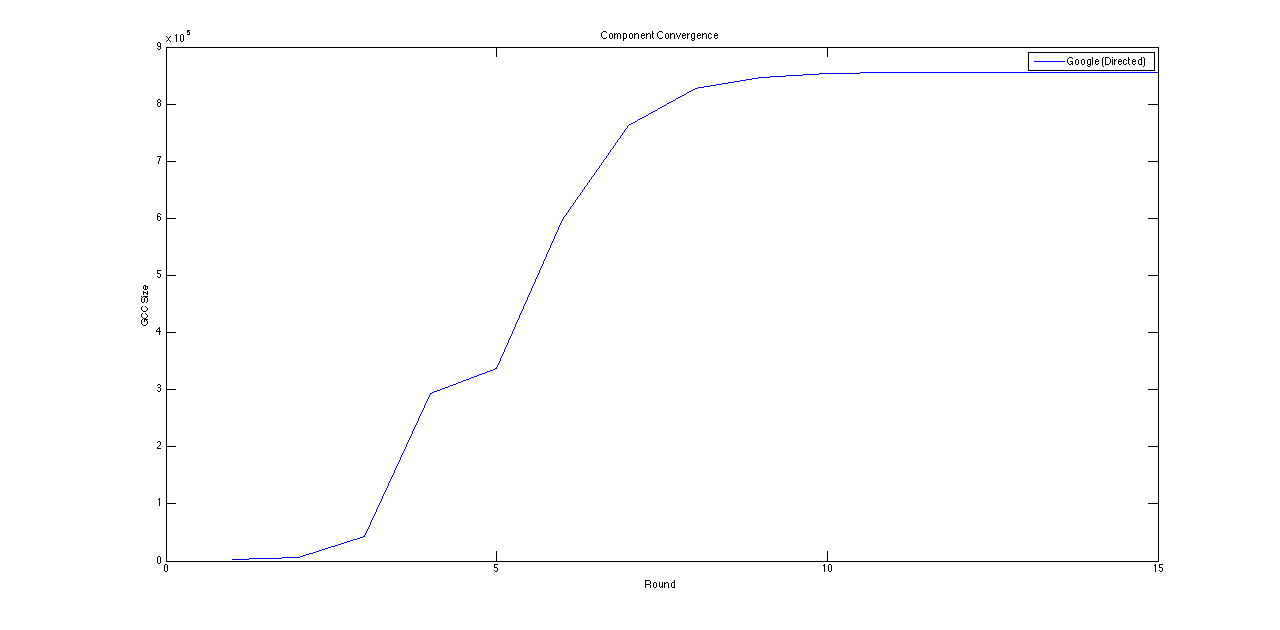
\includegraphics[width=\textwidth]{FIG/cp-google-c.png}
            \caption{Google}
            \label{fig:cp-google-c}
    \end{subfigure}
    ~ %add desired spacing between images, e. g. ~, \quad, \qquad etc.
      %(or a blank line to force the subfigure onto a new line)
    \begin{subfigure}[htbp]{0.8\textwidth}
            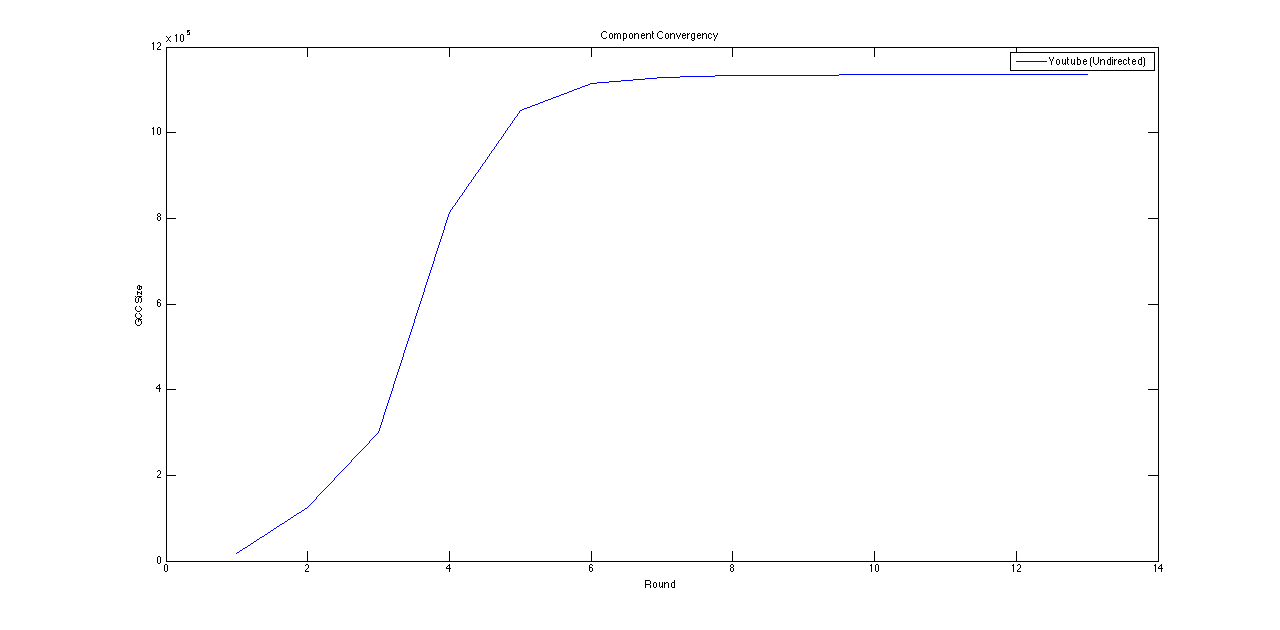
\includegraphics[width=\textwidth]{FIG/cp-youtube-c.png}
            \caption{Youtube}
            \label{fig:cp-youtube-c}
    \end{subfigure}
    ~ %add desired spacing between images, e. g. ~, \quad, \qquad etc.
      %(or a blank line to force the subfigure onto a new line)
    \begin{subfigure}[htbp]{0.8\textwidth}
            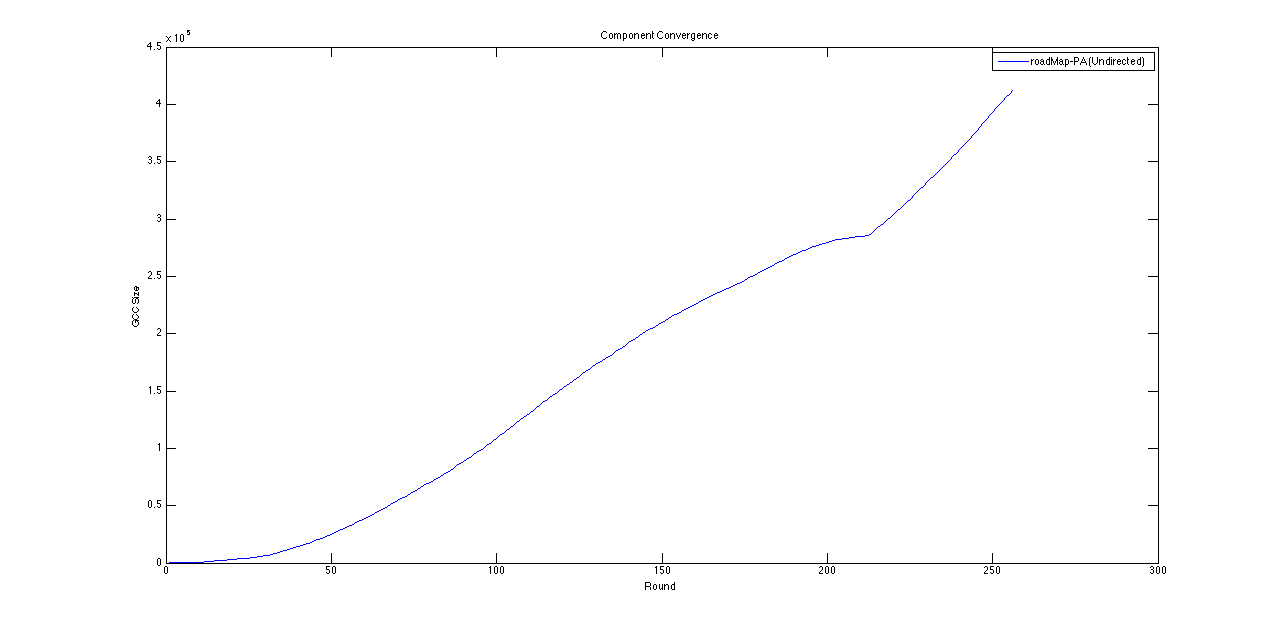
\includegraphics[width=\textwidth]{FIG/cp-pa-c.png}
            \caption{}
            \label{fig:cp-pa-c.png}
    \end{subfigure}
    \caption{Component Convergence}
        \label{fig:results3}
\end{figure} 

We also give the plot of connected component distribution. Notice that Youtube graph is actually all-connected and there is only one GCC. Therefore, we only give the plot of Google, roadMap-PA after 20 iterations, roadMap-PA after 256 iterations(which took over 22000000 ms to run), roadMap-CA after 10 iterations and roadMap-TX after 10 iterations.\\
Figure \ref{fig:results3-1} shows the result of component plot.
\begin{figure}
    \centering
    \begin{subfigure}[htbp]{0.8\textwidth}
            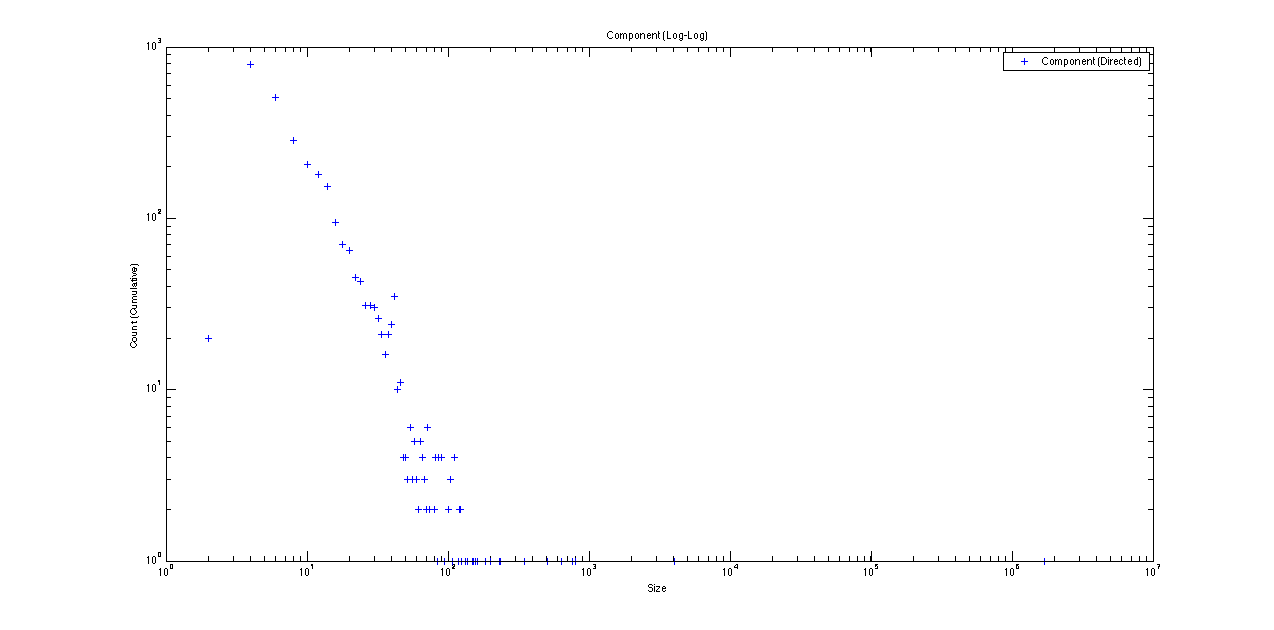
\includegraphics[width=\textwidth]{FIG/cp-google.png}
            \caption{Google}
            \label{fig:cp-google}
    \end{subfigure}
    ~ %add desired spacing between images, e. g. ~, \quad, \qquad etc.
      %(or a blank line to force the subfigure onto a new line)
    \begin{subfigure}[htbp]{0.8\textwidth}
            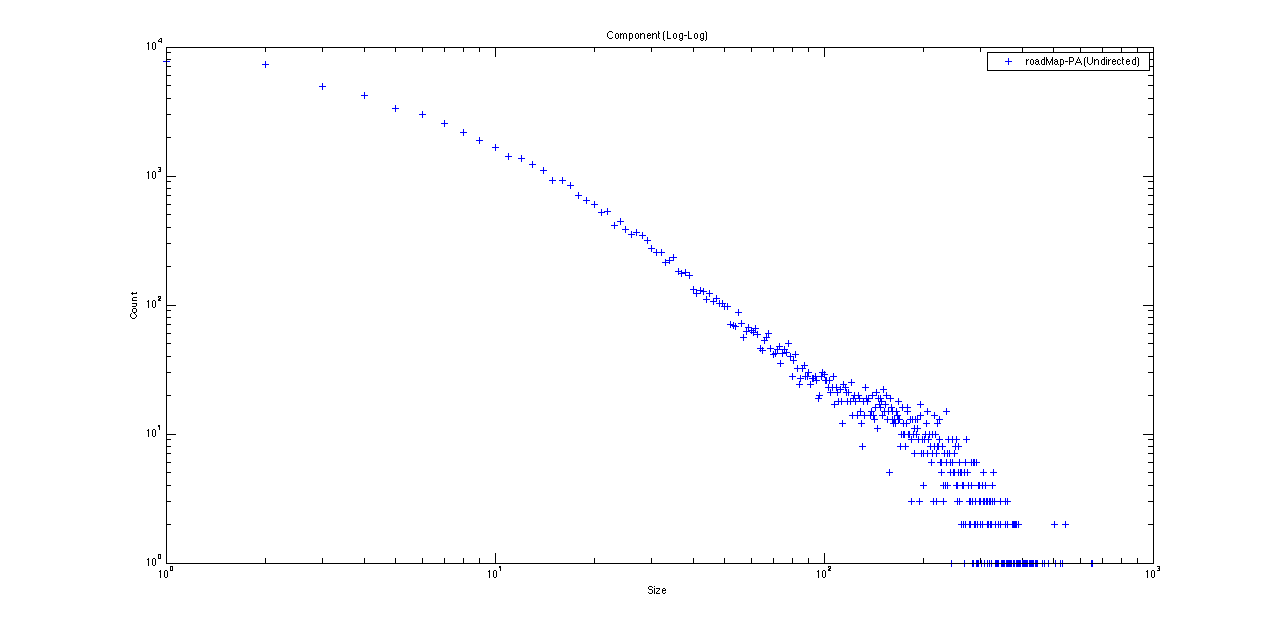
\includegraphics[width=\textwidth]{FIG/cp-pa-20.png}
            \caption{roadMap-PA 20 iterations}
            \label{fig:cp-pa-20}
    \end{subfigure}
    ~ %add desired spacing between images, e. g. ~, \quad, \qquad etc.
      %(or a blank line to force the subfigure onto a new line)
    \begin{subfigure}[htbp]{0.8\textwidth}
            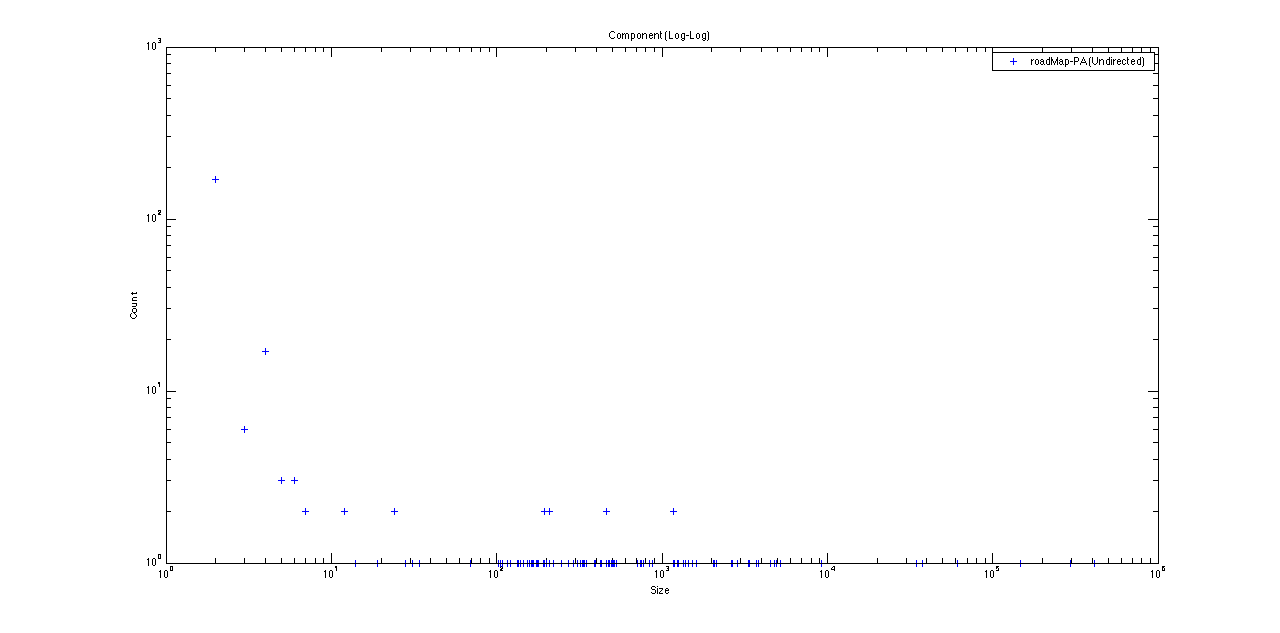
\includegraphics[width=\textwidth]{FIG/cp-pa.png}
            \caption{roadMap-PA 256 iterations}
            \label{fig:cp-pa.png}
    \end{subfigure}
\end{figure}

\addtocounter{figure}{-1}

\begin{figure} 
    \addtocounter{figure}{1}
    \centering 
        % ~ %add desired spacing between images, e. g. ~, \quad, \qquad etc.
          %(or a blank line to force the subfigure onto a new line)
        \begin{subfigure}[htbp]{0.8\textwidth}
                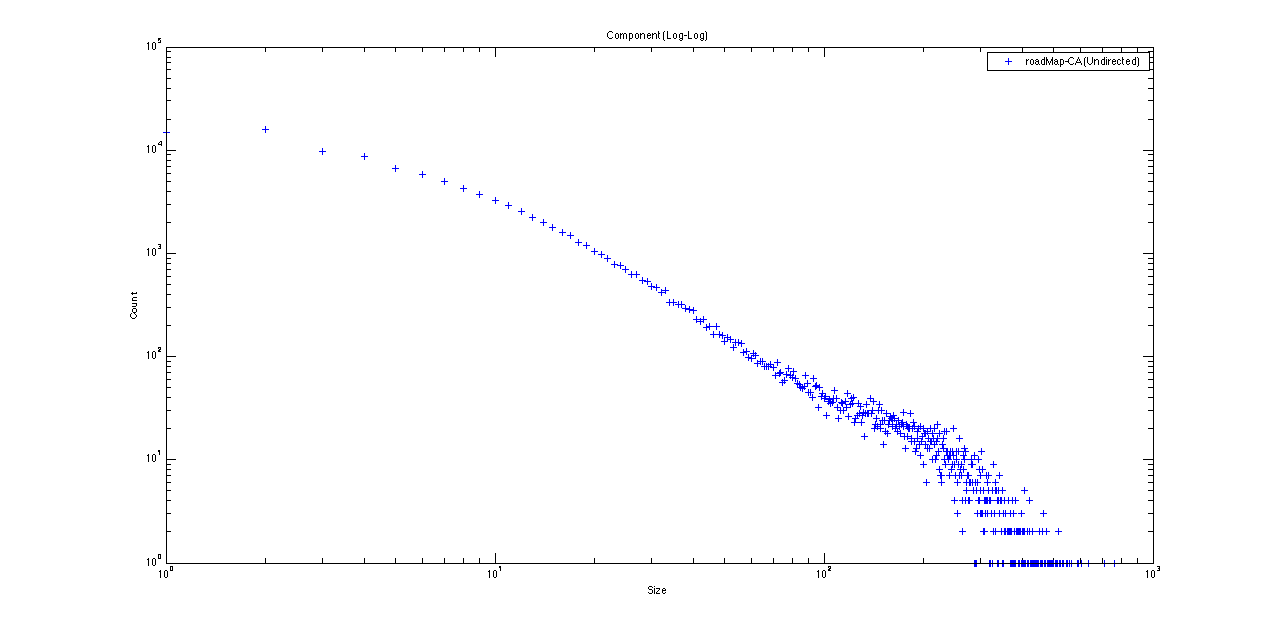
\includegraphics[width=\textwidth]{FIG/cp-ca.png}
                \caption{roadMap-CA 10 iterations}
                \label{fig:cp-pa}
        \end{subfigure}
        ~ %add desired spacing between images, e. g. ~, \quad, \qquad etc.
          %(or a blank line to force the subfigure onto a new line)
        \begin{subfigure}[htbp]{0.8\textwidth}
                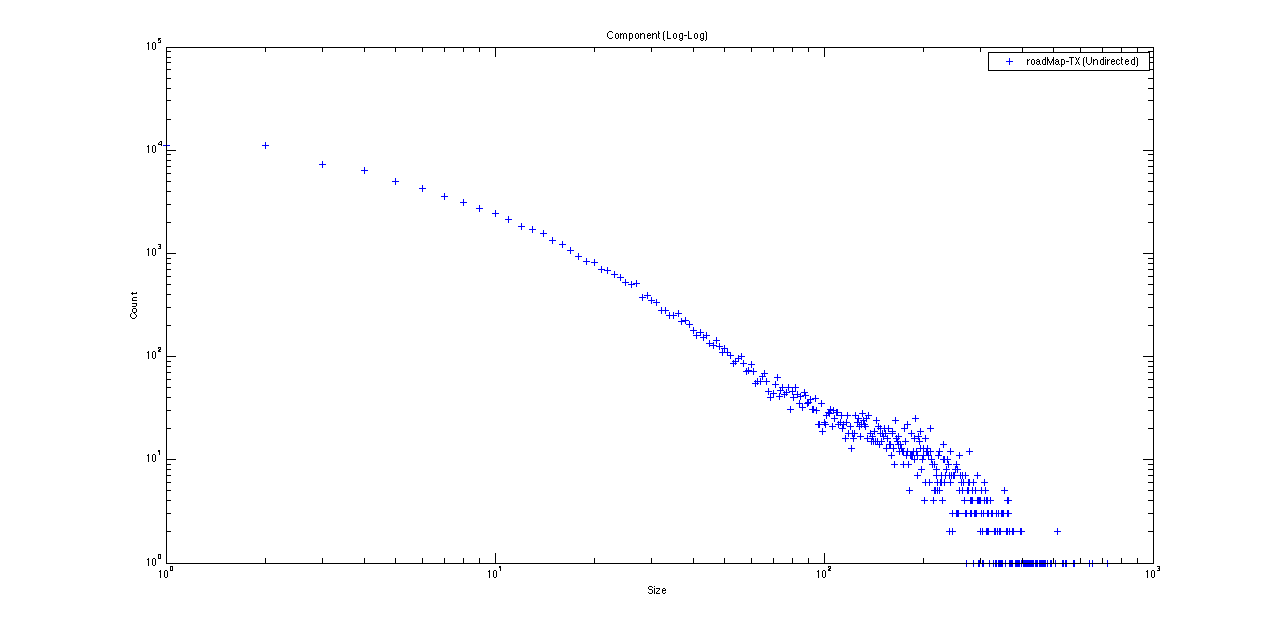
\includegraphics[width=\textwidth]{FIG/cp-tx.png}
                \caption{roadMap-TX 10 iterations}
                \label{fig:cp-tx}
        \end{subfigure}
    \caption{Component Distribution}
    \label{fig:results3-1}
\end{figure} 

%%%%%%%%%%%%%%%%%%%%%%%%%%%%%%%%%%%%%%%%%%%%%%%%%%%%%%%%%%%%%%%%%%%%%%%%%%%%%%%%

\subsection{Task 4: Radius}
\subsubsection{Accuracy Demonstration}
We examine a small test case on a undirected graph with 8 nodes. Figure \ref{fig:results4} shows the graph structire. \\
It is obvious to tell from the image that Node 1 and Node 5 have the largest radium 5, which is the diameter of this graph. \\
Running the algrithm on the graph, we get the output as follows, which is in line with the result from the image.
\begin{verbatim}
postgres=# select * from radius(20);
 node | radius 
------+--------
    1 |      5
    2 |      4
    3 |      3
    4 |      4
    5 |      5
    6 |      2
    7 |      2
    8 |      2
(8 rows)
\end{verbatim}

\begin{figure}[htbf]
\begin{center}
\begin{tabular}{cc}
     % uncomment the next lines, and give the right ps files
     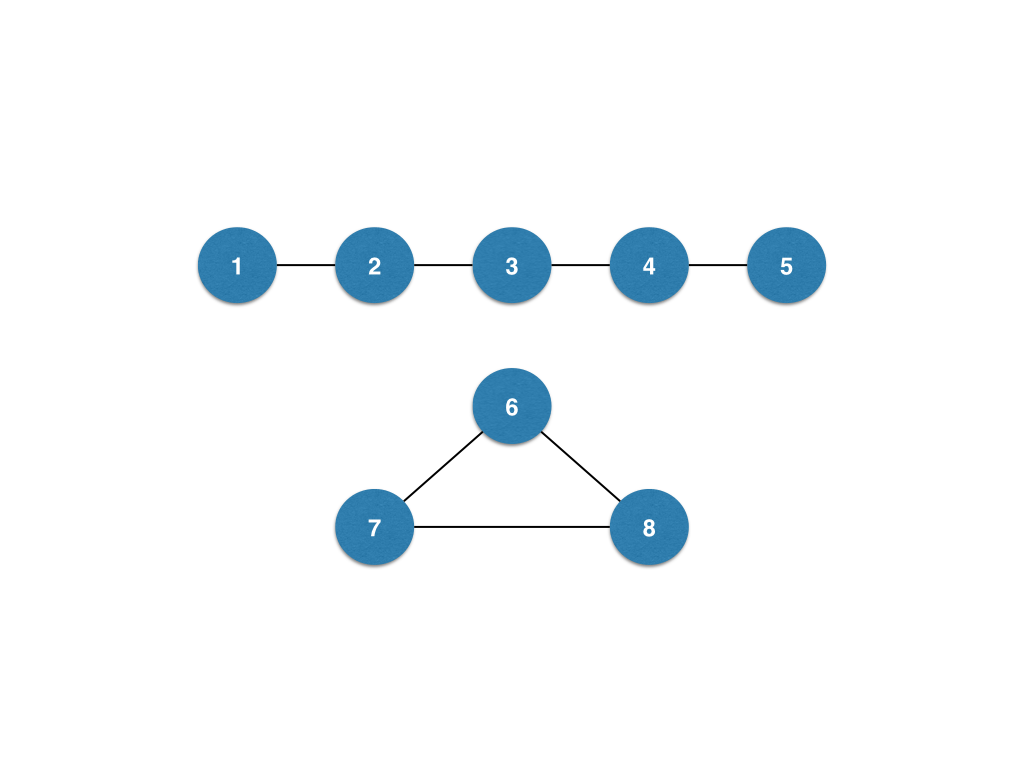
\includegraphics[width=0.6\textwidth]{FIG/task4.png} \\
     %\psfig{figure=FIG/plot.ps,width=2in} \\
     % \psfig{figure=FIG/data.ps,width=2in} &
     % \psfig{figure=FIG/plot.ps,width=2in} \\
\end{tabular}
\caption{Test case graph for Radium and Diameter}
\label{fig:results4}
\end{center}
\end{figure}

\subsubsection{Variety Demonstration}
We perform the test on two 1M node datasets: web-Google(directed) and Youtube. Figure \ref{fig:results3-1} shows the result. \\
Since the iteration stop earlier than maximum iteration(256), we guarantee that radius are converge here. \\
As we mentioned in the last section that real world graphs like road network tend to have chains and large radius, we skip the test here considering its running time.

\begin{figure}
    \centering
    \begin{subfigure}[htbp]{0.8\textwidth}
            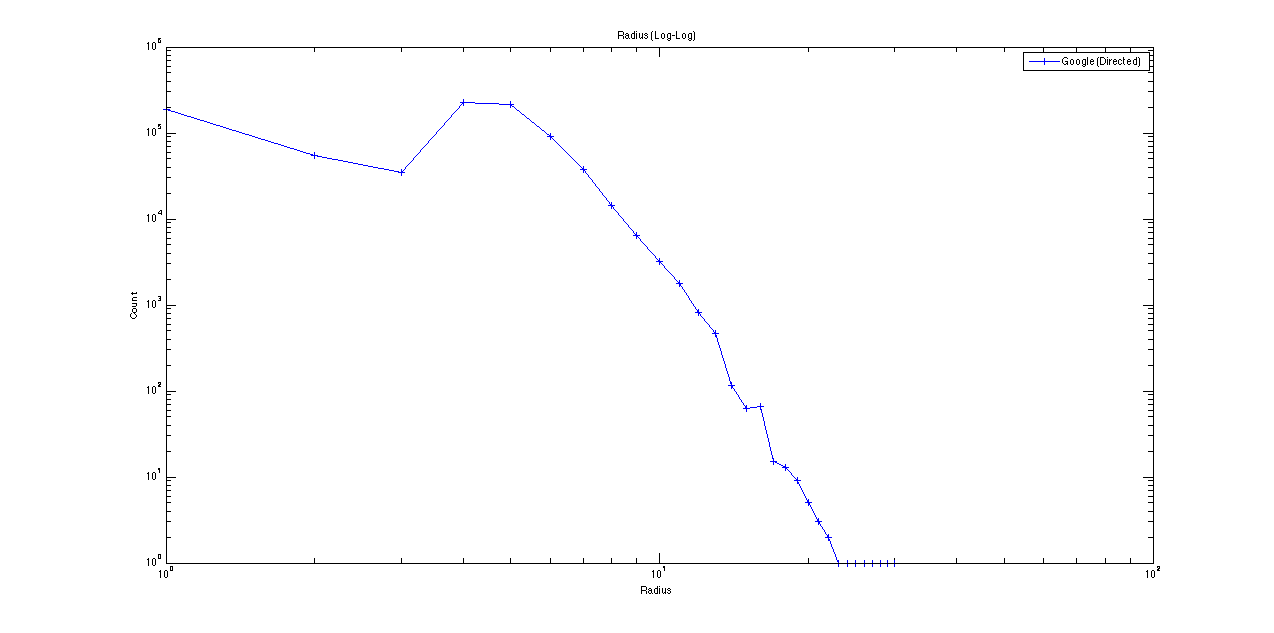
\includegraphics[width=\textwidth]{FIG/rd-google.png}
            \caption{Google}
            \label{fig:rd-google}
    \end{subfigure}
    ~ %add desired spacing between images, e. g. ~, \quad, \qquad etc.
      %(or a blank line to force the subfigure onto a new line)
    \begin{subfigure}[htbp]{0.8\textwidth}
            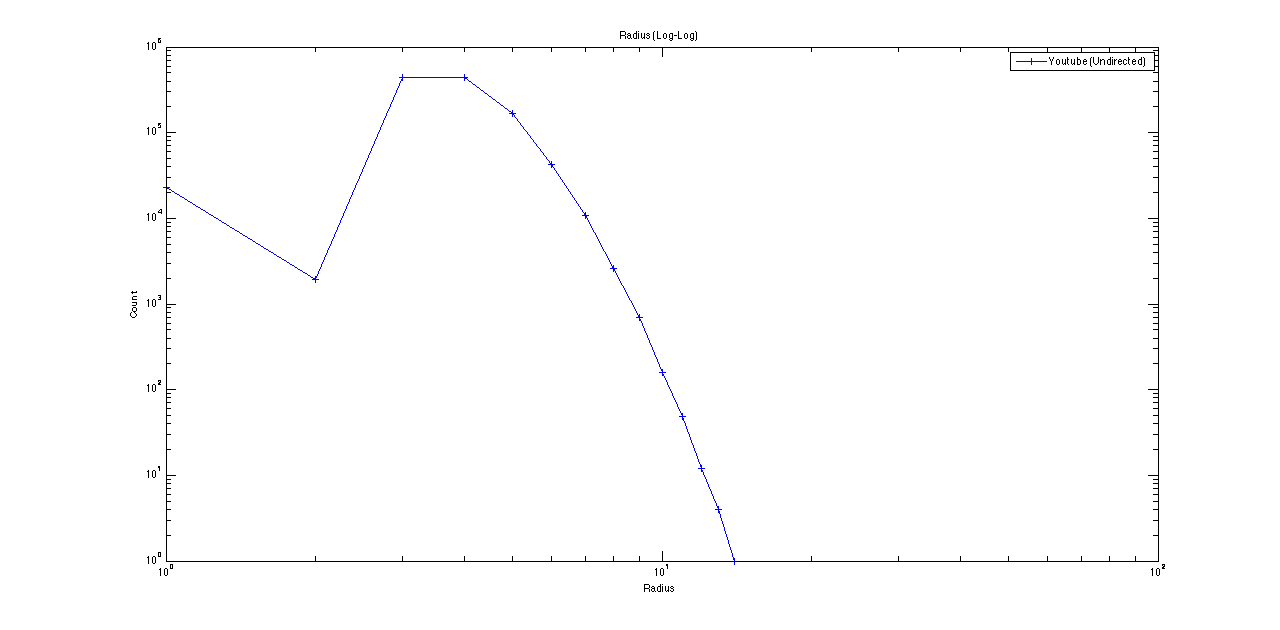
\includegraphics[width=\textwidth]{FIG/rd-youtube.png}
            \caption{Youtube}
            \label{fig:rd-youtube}
    \end{subfigure}
    \caption{Radius Distribution}
        \label{fig:results3-1}
\end{figure}

%%%%%%%%%%%%%%%%%%%%%%%%%%%%%%%%%%%%%%%%%%%%%%%%%%%%%%%%%%%%%%%%%%%%%%%%%%%%%%%%%%%%%%%%%%%%%

\subsection{Task 5: Eigenvalues}
{Accuracy Demonstration}
First, we successfully implemented Lanczos-NO algorithm. But we found there were some eigenvalues missing. We thought it was because the rounding errors from floating-point calculations as its said in the paper. But after we implemented Lanczos-SO algorithm, there are still eigenvalues missing. \\
In the following test, we found out that the correctness of calculating eigenvalues by Lanczos is largely related by the number of iteration and the initial value chosen. The more the number of iteration, the more correctness brought to eigenvalue calculation, but the also the more calculation time it takes. \\
As a treat off, we only calculate the first 10 eigenvalues in the following experiments, as shown in Figure \ref{fig:results5-1}.\\
\begin{figure}[htbf]
\begin{center}
\begin{tabular}{cc}
     % uncomment the next lines, and give the right ps files
     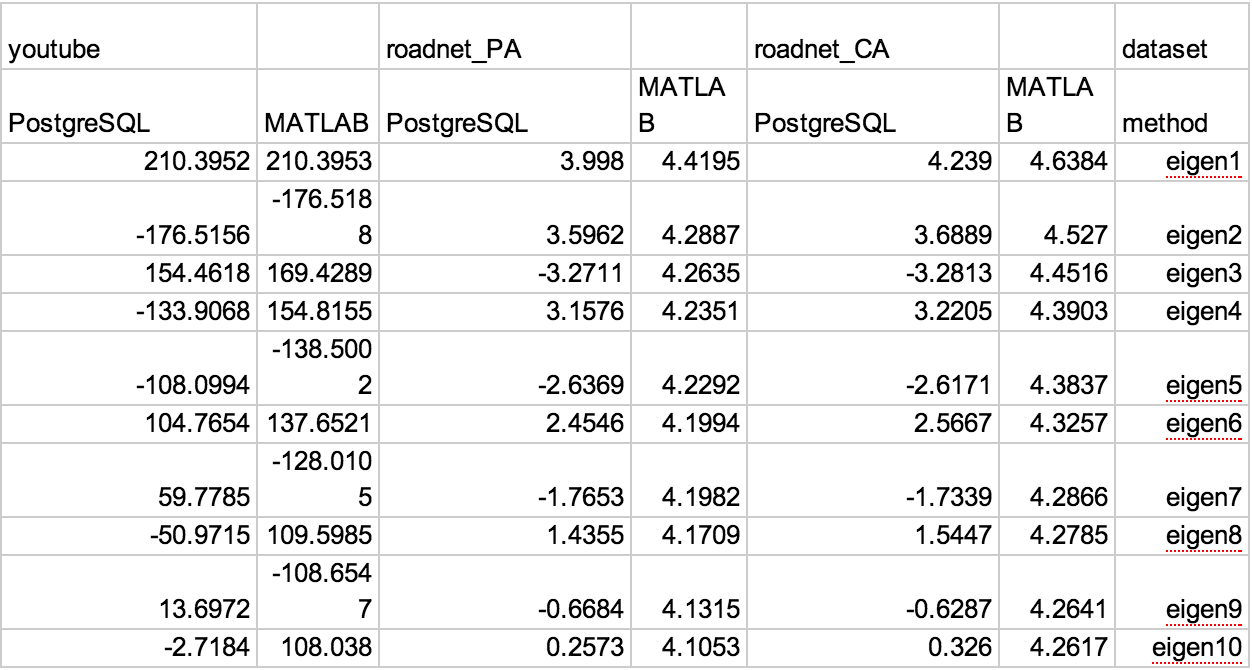
\includegraphics[width=0.8\textwidth]{FIG/tab.png} \\
     %\psfig{figure=FIG/plot.ps,width=2in} \\
     % \psfig{figure=FIG/data.ps,width=2in} &
     % \psfig{figure=FIG/plot.ps,width=2in} \\
\end{tabular}
\caption{Eigenvalues and rank plot}
\label{fig:results5-1}
\end{center}
\end{figure}
As can be seen from the eigenvalues calculated by us and the ones calculated by MATLAB. Only the first few result are corresponding to the greatest eigenvalue that calculated by MATLAB. \\
Our conclusion is that Lanczos algorithm with small number of iteration K, is not suitable to calculate the greatest K eigenvalues of a matrix, because it may not find them all, like the “youtube” dataset. And the calculation result is extremely bad when eigenvalues are close to each other, like “roadnet” datasets. \\
Despite of this, we found out some pattern of the eigenvalues calculated by the Lanczos algorithm. Take a simple dataset - “adjnoun” - as example. The eigenvalue-rank plot is as follows in Figure \ref{fig:results5}. \\
As can be seen in the graph, the first few eigenvalues are alternately greater or smaller than 0, and the absolute value of eigenvalues are getting smaller.

\begin{figure}[htbf]
\begin{center}
\begin{tabular}{cc}
     % uncomment the next lines, and give the right ps files
     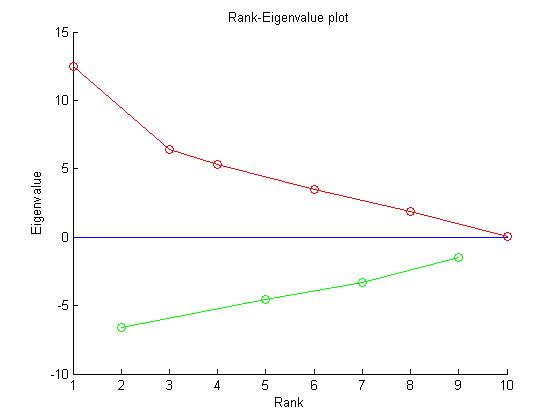
\includegraphics[width=0.8\textwidth]{FIG/task5.jpg} \\
     %\psfig{figure=FIG/plot.ps,width=2in} \\
     % \psfig{figure=FIG/data.ps,width=2in} &
     % \psfig{figure=FIG/plot.ps,width=2in} \\
\end{tabular}
\caption{Eigenvalues-rank plot for adjnoun dataset}
\label{fig:results5}
\end{center}
\end{figure}

\subsubsection{Varienty Demonstration}
We perform the test on several 1M nodes datasets: social-Youtube, roadMap-PA and roadMap-CA. Figure \ref{fig:results5-2} shows the result.\\
\begin{figure}
    \centering
    \begin{subfigure}[htbp]{0.6\textwidth}
            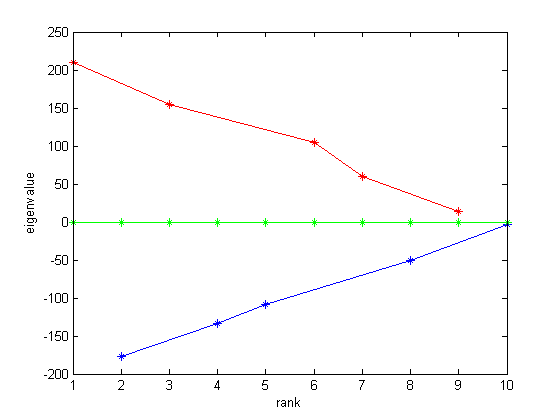
\includegraphics[width=\textwidth]{FIG/ei-youtube.png}
            \caption{Youtube}
            \label{fig:ei-youtube}
    \end{subfigure}
    ~ %add desired spacing between images, e. g. ~, \quad, \qquad etc.
      %(or a blank line to force the subfigure onto a new line)
    \begin{subfigure}[htbp]{0.6\textwidth}
            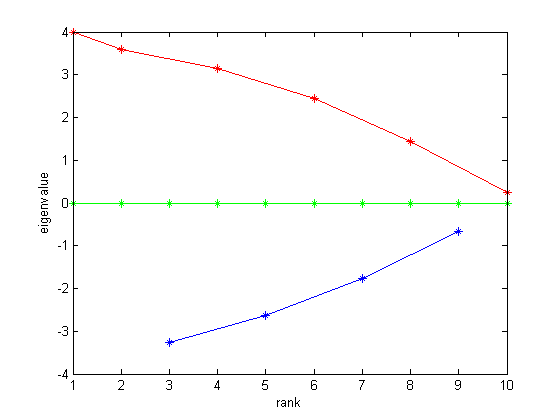
\includegraphics[width=\textwidth]{FIG/ei-pa.png}
            \caption{roadMap-PA}
            \label{fig:ei-pa}
    \end{subfigure}
    ~ %add desired spacing between images, e. g. ~, \quad, \qquad etc.
      %(or a blank line to force the subfigure onto a new line)
    \begin{subfigure}[htbp]{0.6\textwidth}
            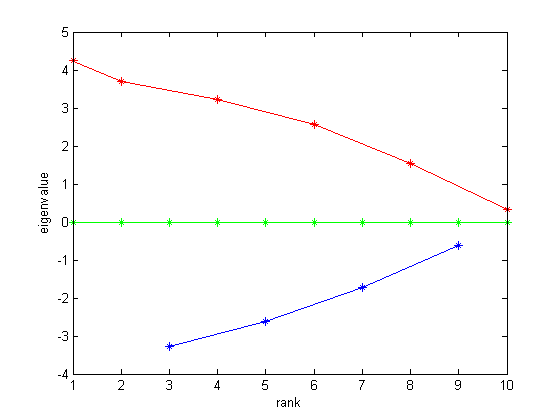
\includegraphics[width=\textwidth]{FIG/ei-ca.png}
            \caption{roadMap-CA}
            \label{fig:ei-ca.png}
    \end{subfigure}
    \caption{Eigenvalues and rank plot}
        \label{fig:results5-2}
\end{figure} 

%%%%%%%%%%%%%%%%%%%%%%%%%%%%%%%%%%%%%%%%%%%%%%%%%%%%%%%%%%%%%%%%%%%%%%%%%%%%%%%%%%

\subsection{Task 6: Belief Propagation}
\subsubsection{Accuracy Demonstration}
First, We want to check if the algorithm is able to give the correct inference of unlabed node. \\
We examine a small test case on a undirected graph with 4 nodes. Figure \ref{fig:results6} shows the graph structure. Given the label and initial belief of node 1, 2, 3, we intend to infer the label of node 4. \\
As for the intial belief, we set node 1=0.4(label: +), node 2=-0.4(label: -), node 3=0.3(label: +), and we leave node 4 = 0(lable: unknown). From the architecture of the graph, we can easily reach the conclusion that node 4 is more likely to be labeled as +(i.e. belief(node 4) > 0).\\
After performing the FastBP algorithm on the test graph, we have the output as follows. The node 4 is classified as +, which is what we expect.

\begin{verbatim}
postgres=# SELECT * from bp(20);
 v_row |       v_val        
-------+--------------------
     1 |  0.273209372007041
     2 | -0.198949408545921
     3 |  0.159512788522935
     4 | 0.0141145717811318
(4 rows)
\end{verbatim}

One thing worths noticing is that as $h_h$ serve as “about-half” homophily factor according to FastBP paper\cite{koutra2011unifying}. $h_h$ close to -0.5 means strong heterophily, while $h_h$ close to 0.5 means strong homophily. Therefore, we can also heterophily inference on the graph by setting $h_h$ to be negative.\\
Second, we want to check if the algorithm can converge. We compare the result after 10 iterations, 50 iterations and 100 iterations, which shows that the FastBP algorithm does converge.

\begin{verbatim}
10 iterations:
 v_row |         v_val         
-------+-----------------------
     1 |     0.288775545358658
     2 |    -0.264187325537205
     3 |     0.222905980050564
     4 | -0.000686401128768922

50 iterations:
 v_row |       v_val        
-------+--------------------
     1 |  0.273209372007041
     2 | -0.198949408545921
     3 |  0.159512788522935
     4 | 0.0141145717811318

100 iterations:
 v_row |       v_val        
-------+--------------------
     1 |  0.272932111246243
     2 | -0.197774913230647
     3 |  0.158338293512337
     4 | 0.0143918324157287
\end{verbatim}

\begin{figure}[htbf]
\begin{center}
\begin{tabular}{cc}
     % uncomment the next lines, and give the right ps files
     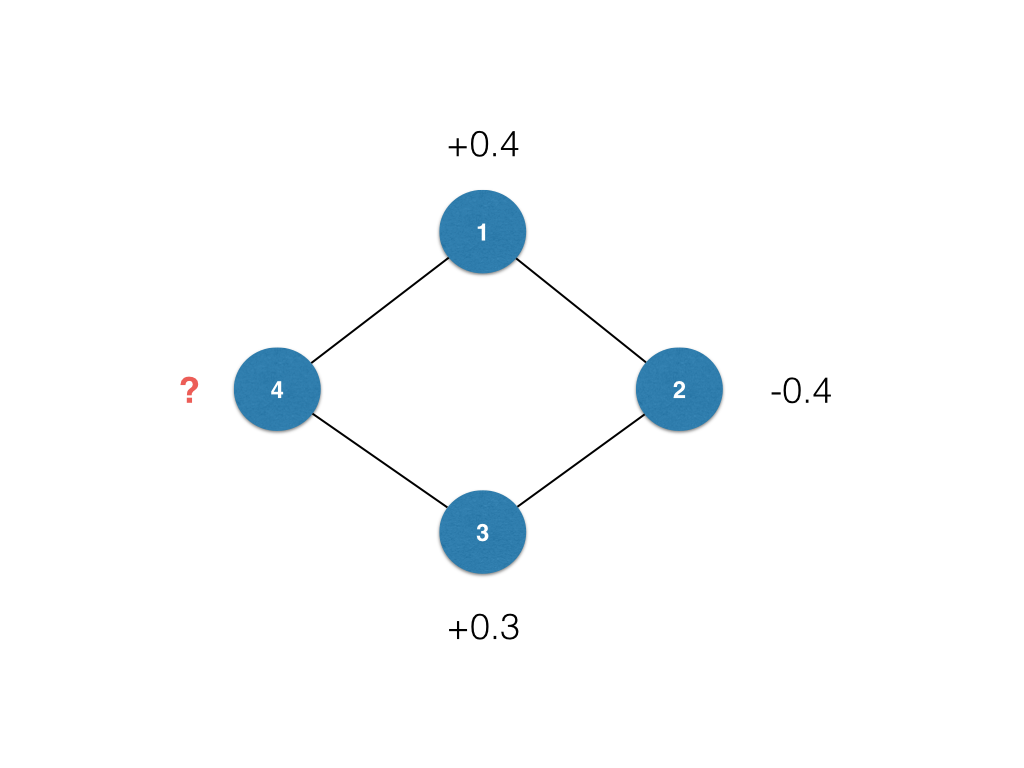
\includegraphics[width=0.6\textwidth]{FIG/task6.png} \\
     %\psfig{figure=FIG/plot.ps,width=2in} \\
     % \psfig{figure=FIG/data.ps,width=2in} &
     % \psfig{figure=FIG/plot.ps,width=2in} \\
\end{tabular}
\caption{Test case graph for Belief Propagation}
\label{fig:results6}
\end{center}
\end{figure}

\subsubsection{Varienty Demonstration}
We perform the test on five 1M node datasets: web-Google(directed), social-Youtube, roadMap-PA, roadMap-CA, and roadMap-TX. As for initialization, we set the prior belief to 0.01 for all nodes. \\
Figure \ref{fig:results6-1} shows the result.\\
Notice that we are using cumulative count here in terms of the y-axis. That is, while x is the belief of a specific point, y is the number of points with greater belief value than that point.

\begin{figure}
    \centering
    \begin{subfigure}[htbp]{0.9\textwidth}
            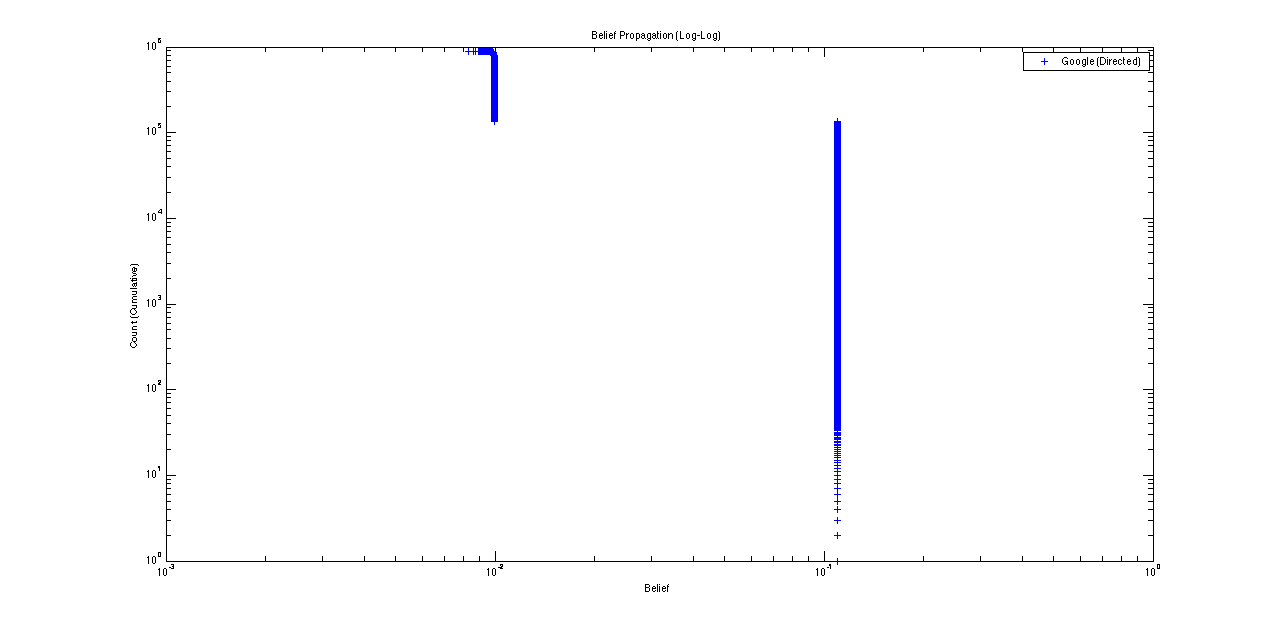
\includegraphics[width=\textwidth]{FIG/bp-google.png}
            \caption{Google}
            \label{fig:bp-google}
    \end{subfigure}
    ~ %add desired spacing between images, e. g. ~, \quad, \qquad etc.
      %(or a blank line to force the subfigure onto a new line)
    \begin{subfigure}[htbp]{0.9\textwidth}
            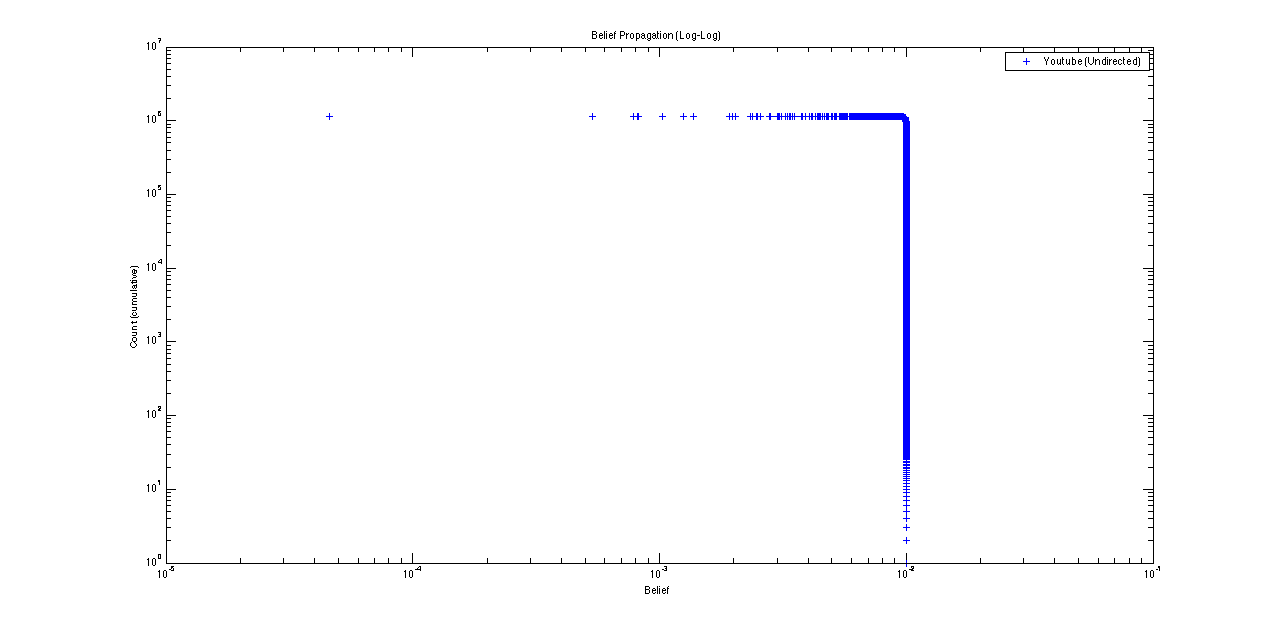
\includegraphics[width=\textwidth]{FIG/bp-youtube.png}
            \caption{Youtube}
            \label{fig:bp-youtube}
    \end{subfigure}
\end{figure} 

\addtocounter{figure}{-1}

\begin{figure} 
    \addtocounter{figure}{1}
    \centering 
        % ~ %add desired spacing between images, e. g. ~, \quad, \qquad etc.
          %(or a blank line to force the subfigure onto a new line)
        \begin{subfigure}[htbp]{0.9\textwidth}
                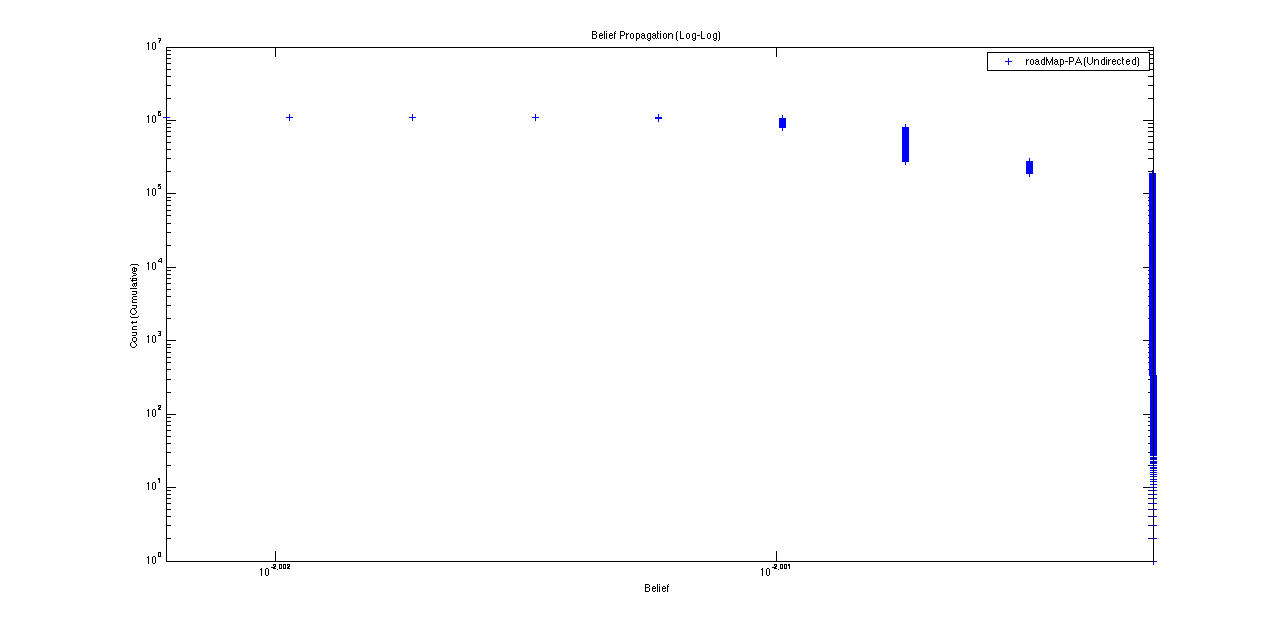
\includegraphics[width=\textwidth]{FIG/bp-pa.png}
                \caption{roadMap-PA}
                \label{fig:bp-pa}
        \end{subfigure}
        ~ %add desired spacing between images, e. g. ~, \quad, \qquad etc.
          %(or a blank line to force the subfigure onto a new line)
        \begin{subfigure}[htbp]{0.9\textwidth}
                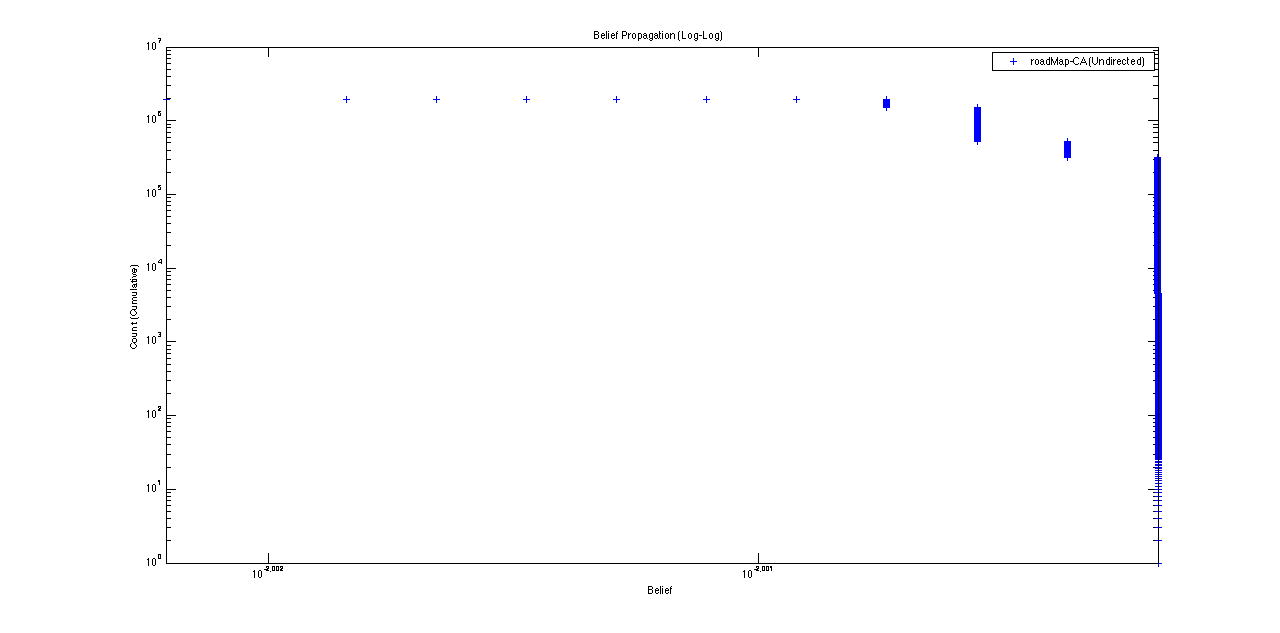
\includegraphics[width=\textwidth]{FIG/bp-ca.png}
                \caption{roadMap-CA}
                \label{fig:bp-ca}
        \end{subfigure}
        ~ %add desired spacing between images, e. g. ~, \quad, \qquad etc.
          %(or a blank line to force the subfigure onto a new line)
        \begin{subfigure}[htbp]{0.9\textwidth}
                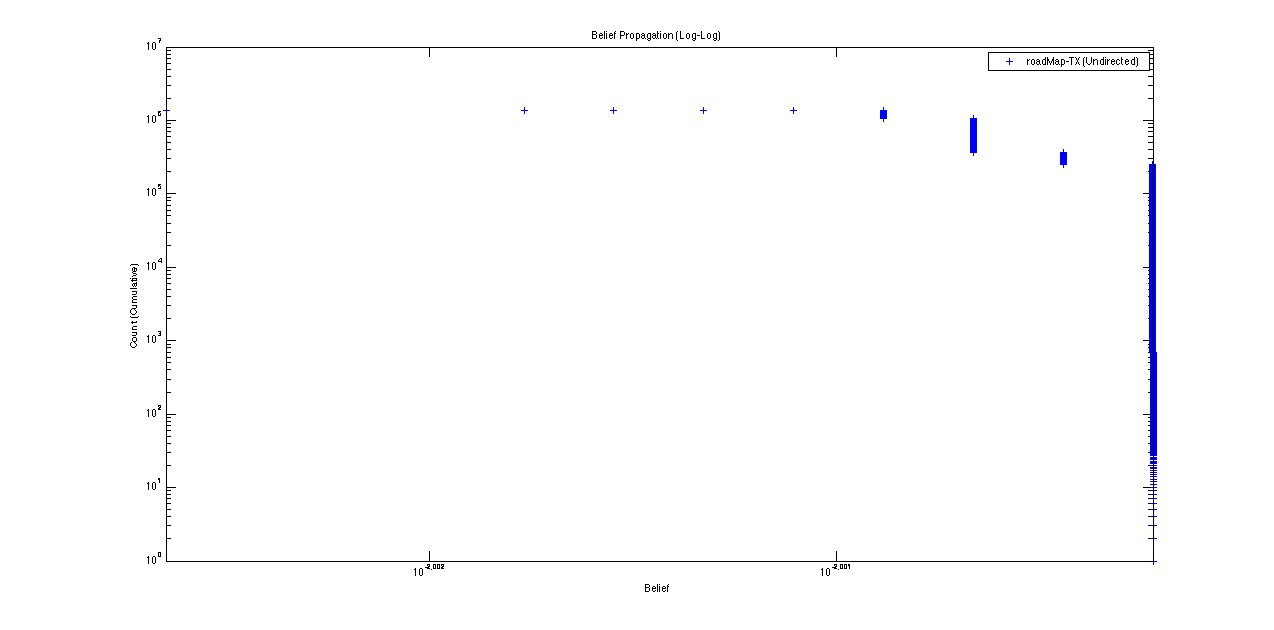
\includegraphics[width=\textwidth]{FIG/bp-tx.png}
                \caption{roadMap-TX}
                \label{fig:bp-tx}
        \end{subfigure}
        \caption{Belief Distribution}
        \label{fig:results6-1}
\end{figure}


%%%%%%%%%%%%%%%%%%%%%%%%%%%%%%%%%%%%%%%%%%%%%%%%%%%%%%%%%%%%%%%%%%%%%%%%%%%%%%%%%%
\subsection{Task 7: Count of Triangles}
\subsubsection{Accuracy Demonstration}
As we talked about in task 5, the eigenvalues calculated by Lanczos-SO are not all the eigenvalues of the adjacency matrix nor are the greatest values. As we do the experiment, the triangle counting are not accurate because of this. \\
The experiment result is as follow in Figure \ref{fig:results7}.\\
As can be seen by comparing the result of PostgreSQL implementation and MATLAB, the count of triangle has some difference. This is because the Lanczos algorithm we implemented failed to find out all the greatest eigenvalue. \\
But they all have the same pattern, that is, subject to the power law. There are a great many of nodes that have small number of triangle and a few number of nodes that have very large number of triangle.\\
From the computation from MATLAB, we can see that there are about 10 nodes with extremely large number of triangles, that maybe the super star on youtube website. \\
And there are stand out phenomenon at around triangle number 100. This may because there are certain youtube groups of people that they all know each other in the same group.

\begin{figure}
    \centering
    \begin{subfigure}[htbp]{0.8\textwidth}
            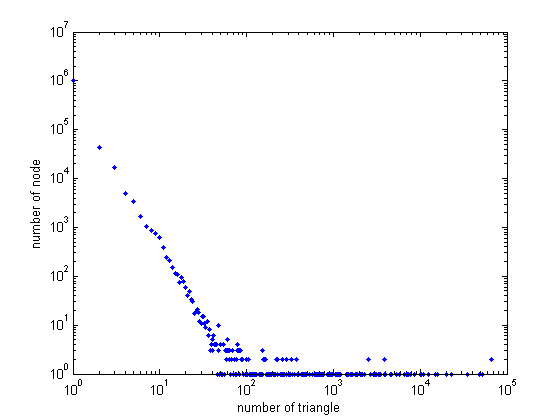
\includegraphics[width=\textwidth]{FIG/my_youtube_triangle.png}
            \caption{Youtube: Triangle Distribution}
            \label{fig:my_youtube_triangle}
    \end{subfigure}
    ~ %add desired spacing between images, e. g. ~, \quad, \qquad etc.
      %(or a blank line to force the subfigure onto a new line)
    \begin{subfigure}[htbp]{0.8\textwidth}
            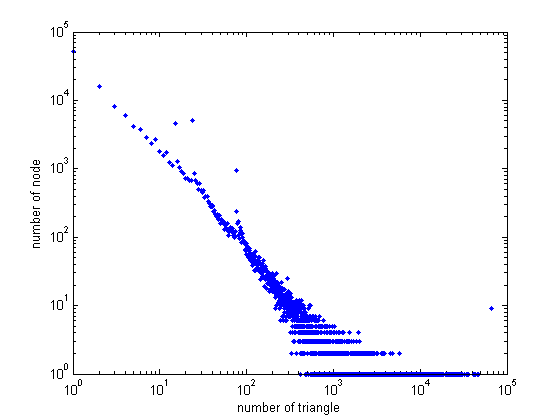
\includegraphics[width=\textwidth]{FIG/matlab_youtube_triangle.png}
            \caption{Youtube: Triangle Distribution(Matlab)}
            \label{fig:matlab}
    \end{subfigure}
    \caption{Weight/Triangle Distribution}
        \label{fig:results7}
\end{figure}

\subsubsection{Variety Demonstration}
We perform the test on 1M nodes social-Youtube dataset. From \ref{fig:results7}, we observes the ’triangle partic- ipation’ law (TPL).

%%%%%%%%%%%%%%%%%%%%%%%%%%%%%%%%%%%%%%%%%%%%%%%%%%%%%%%%%%%%%%%%%%%%%%%%%%%%%%%%%%
 \subsection{Task 8: Innovation Task}
 As we mentioned in the method section, we intend to extend algorithms to directed graph and weighted graph. As for directed graph, we have alread given the plot of web-Google graph in the variety sections of abbove related tasks. \\
 Here we will cover the case of weighted degree distribution and weighted PageRank distribution. The graph we use is Libimseti dataset.\\
 First we give the plot of in/out-degree and in/out weight as follows in Figure \ref{fig:results8}. \\
\begin{figure} 
    \centering 
        % ~ %add desired spacing between images, e. g. ~, \quad, \qquad etc.
          %(or a blank line to force the subfigure onto a new line)
        \begin{subfigure}[htbp]{0.6\textwidth}
                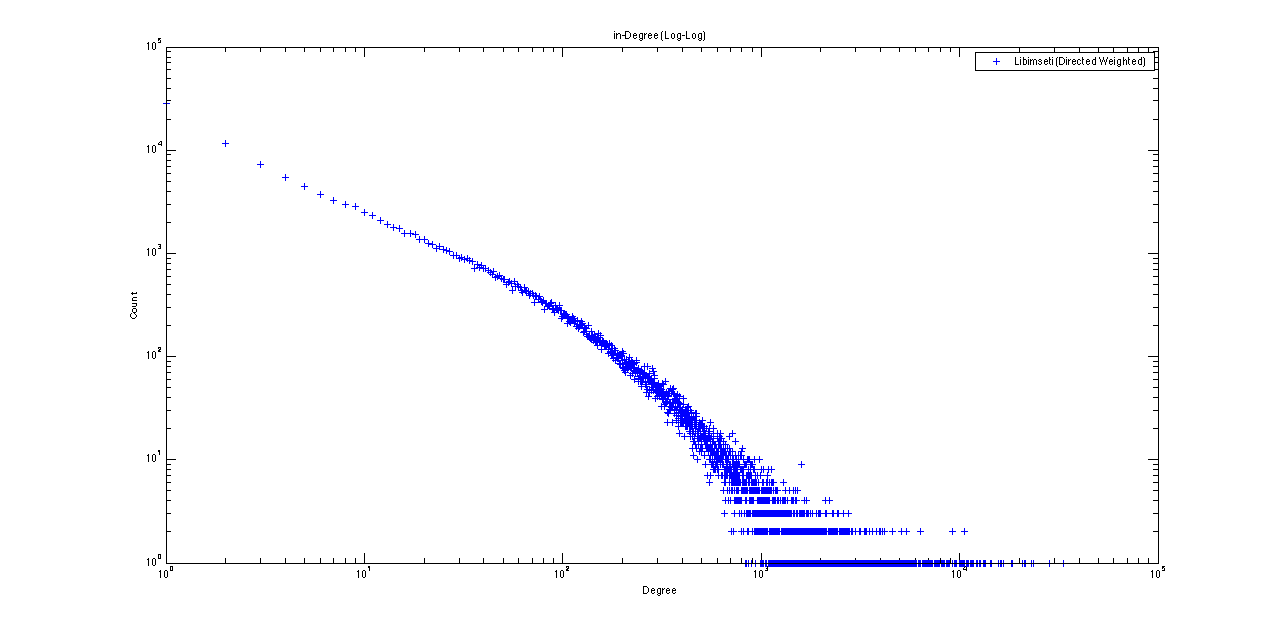
\includegraphics[width=\textwidth]{FIG/dw_ind.png}
                \caption{Libimseti in-Degree}
                \label{fig:dw_ind}
        \end{subfigure} %
        ~ %add desired spacing between images, e. g. ~, \quad, \qquad etc.
          %(or a blank line to force the subfigure onto a new line)
        \begin{subfigure}[htbp]{0.6\textwidth}
                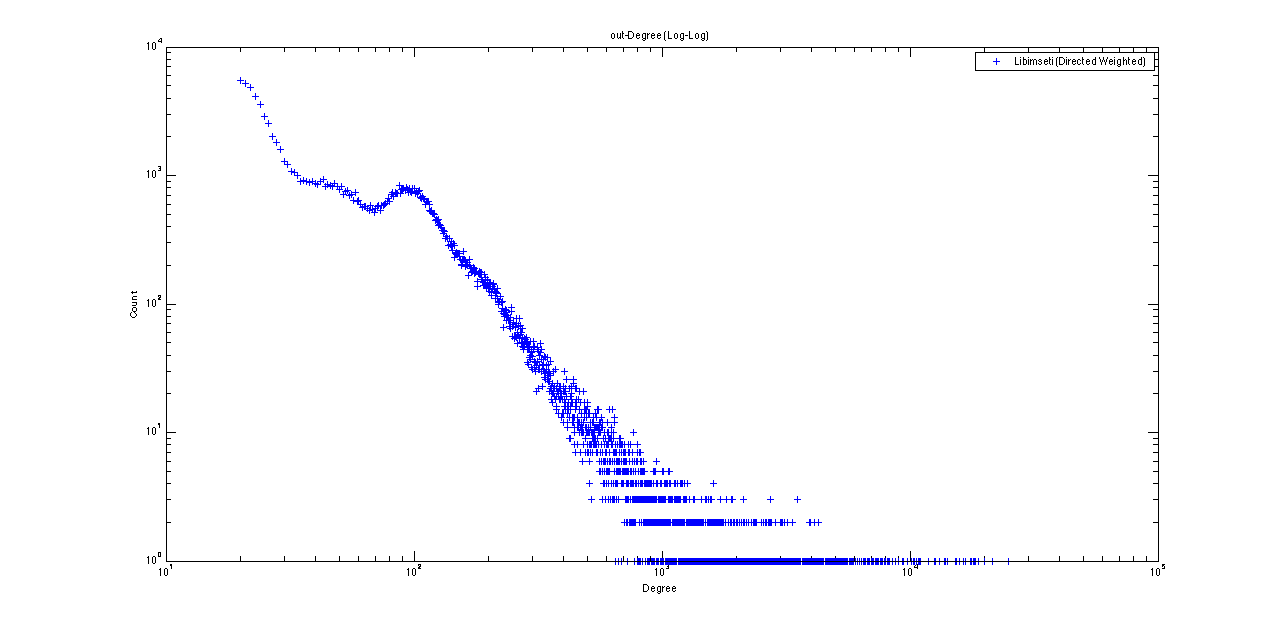
\includegraphics[width=\textwidth]{FIG/dw_outd.png}
                \caption{Libimseti out-Degree}
                \label{fig:dw_outd}
        \end{subfigure}
        ~ %add desired spacing between images, e. g. ~, \quad, \qquad etc.
          %(or a blank line to force the subfigure onto a new line)
        \begin{subfigure}[htbp]{0.6\textwidth}
                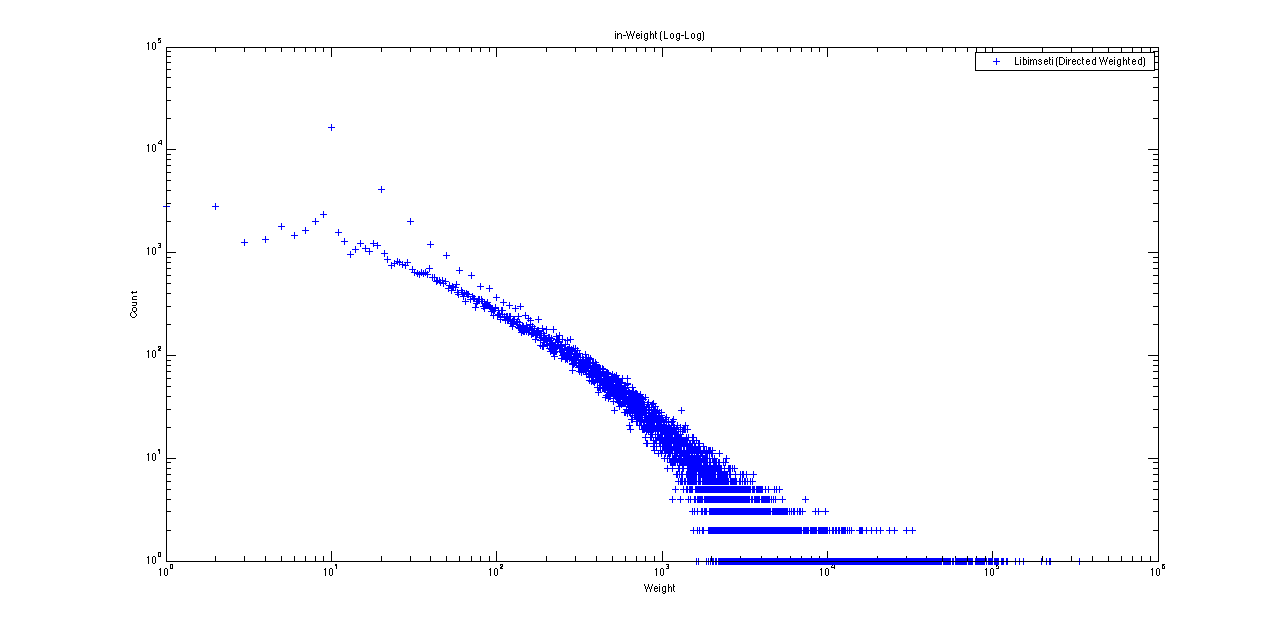
\includegraphics[width=\textwidth]{FIG/dw_inw.png}
                \caption{Libimseti in-Weight}
                \label{fig:dw_inw}
        \end{subfigure} %
        ~ %add desired spacing between images, e. g. ~, \quad, \qquad etc.
          %(or a blank line to force the subfigure onto a new line)
        \begin{subfigure}[htbp]{0.6\textwidth}
                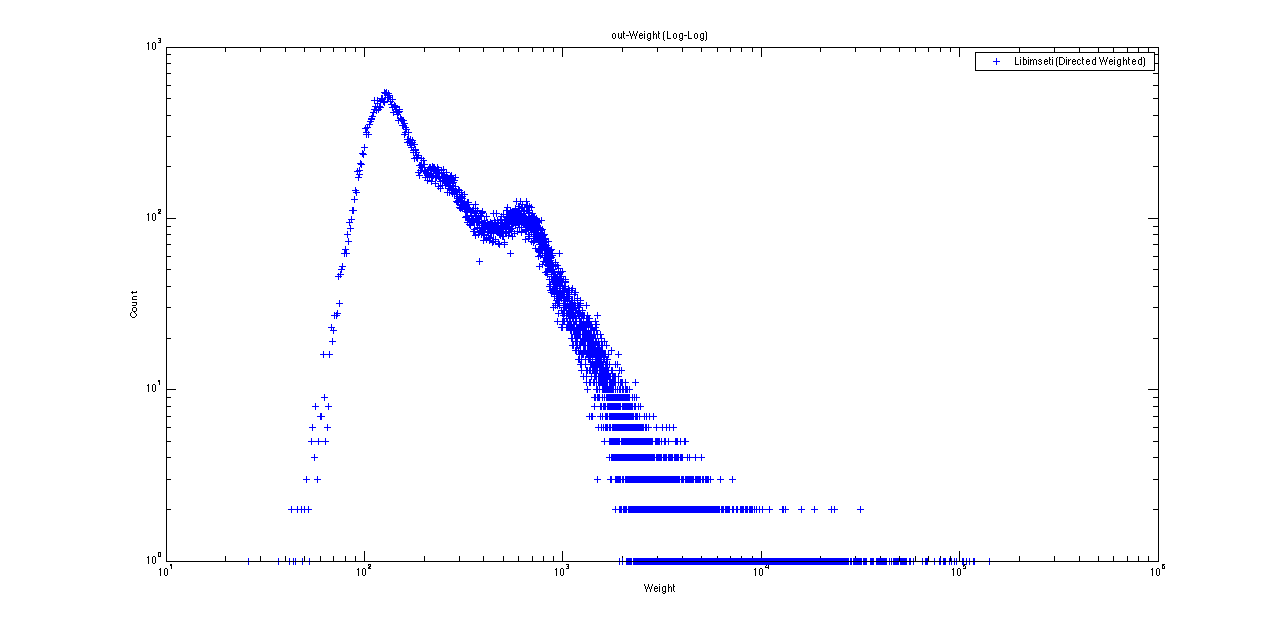
\includegraphics[width=\textwidth]{FIG/dw_outw.png}
                \caption{Libimseti out-Weight}
                \label{fig:dw_outw}
        \end{subfigure}
        \caption{Weight and Degree Distribution}
        \label{fig:results8}
\end{figure}
Then we plot in-weight and in-degree together as well as out-weight and out-degree together in Figure \ref{fig:results8-1}, which shows the SNAPSHOT POWER LAWS (SPL). \\

\begin{figure}
    \centering
    \begin{subfigure}[htbp]{0.8\textwidth}
            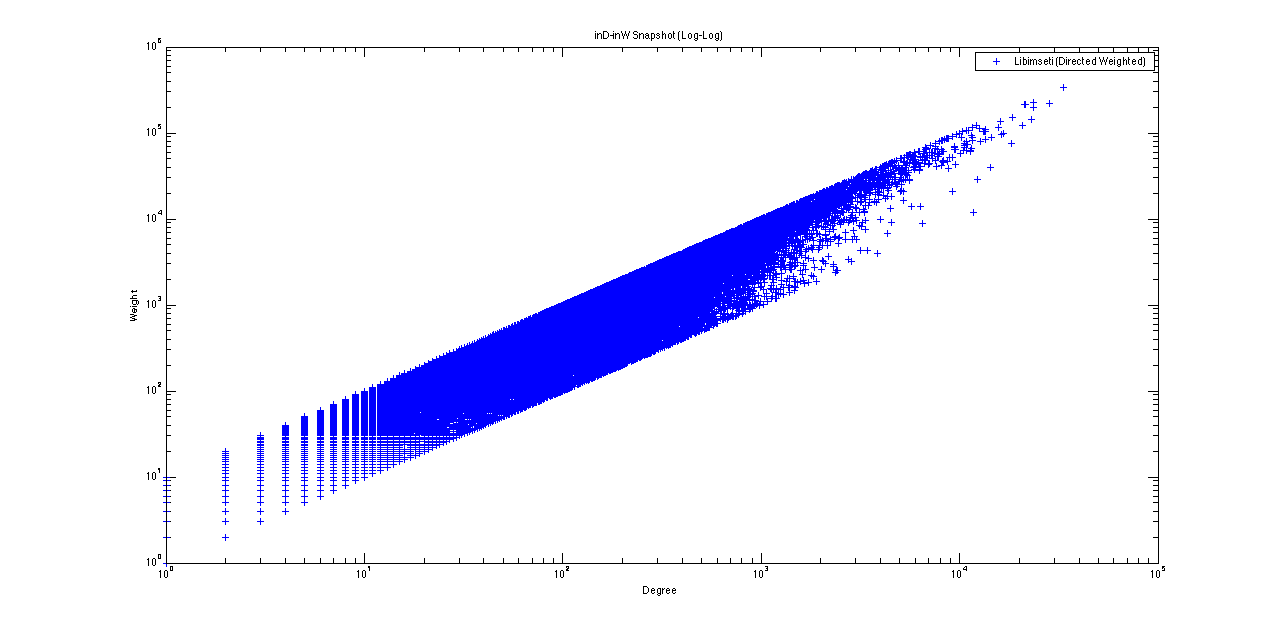
\includegraphics[width=\textwidth]{FIG/dw_in.png}
            \caption{inD-inW snapshot}
            \label{fig:dw-out}
    \end{subfigure}
    ~ %add desired spacing between images, e. g. ~, \quad, \qquad etc.
      %(or a blank line to force the subfigure onto a new line)
    \begin{subfigure}[htbp]{0.8\textwidth}
            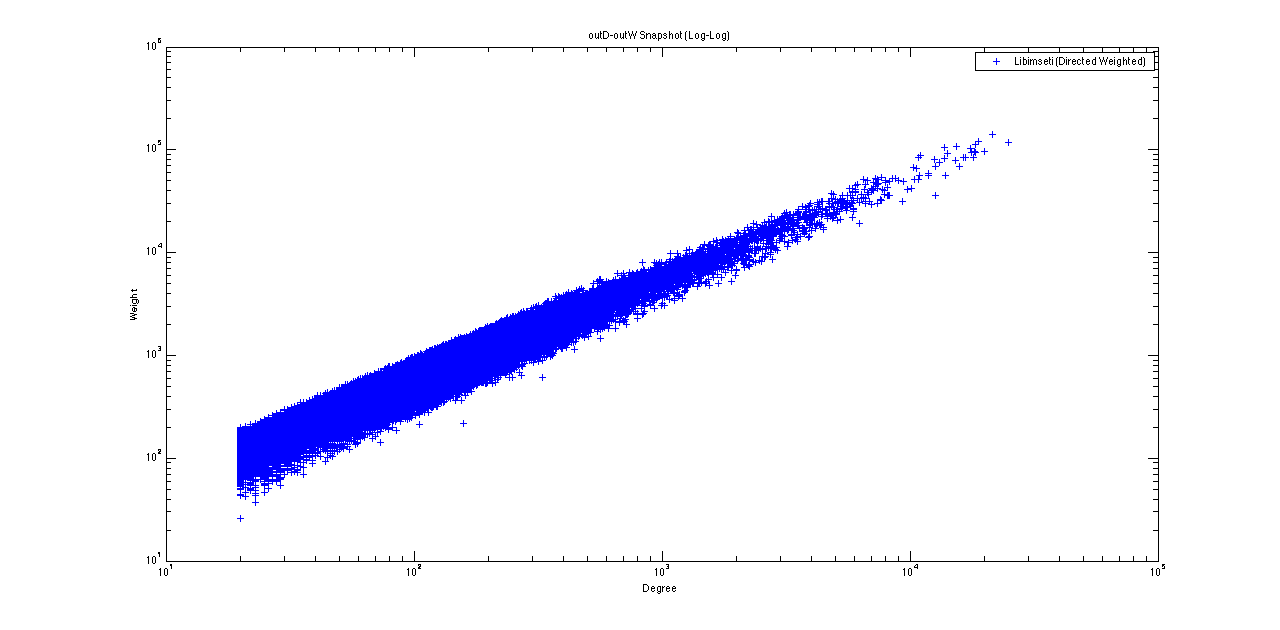
\includegraphics[width=\textwidth]{FIG/dw_out.png}
            \caption{outD-outW snapshot}
            \label{fig:dw-out}
    \end{subfigure}
    \caption{Weight/Degree Snapshot}
        \label{fig:results8-1}
\end{figure}

Finally, we give the plot of PageRank distribution and distributed PageRank distribution. From Figure \ref{fig:results8-2}, we can figure out that both of graphs follow the power law distribution and they are very similar to each other.
\begin{figure}
    \centering
    \begin{subfigure}[htbp]{0.8\textwidth}
            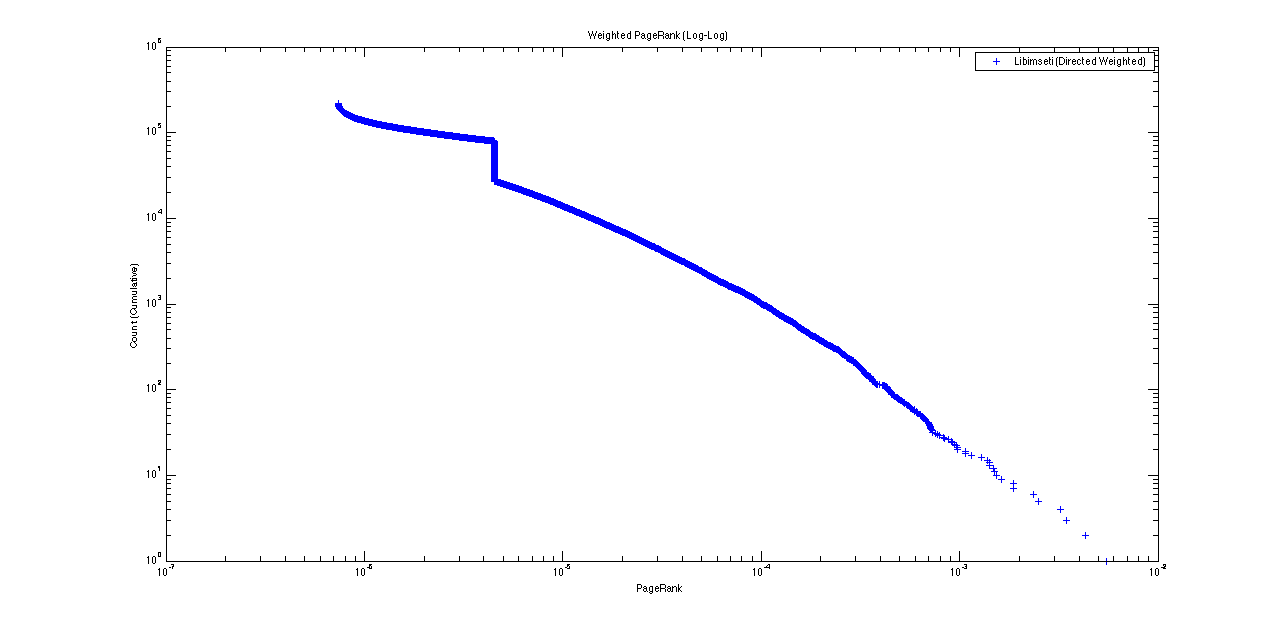
\includegraphics[width=\textwidth]{FIG/dw_pr.png}
            \caption{Weighted PageRank Distribution}
            \label{fig:dw-pr}
    \end{subfigure}
    ~ %add desired spacing between images, e. g. ~, \quad, \qquad etc.
      %(or a blank line to force the subfigure onto a new line)
    \begin{subfigure}[htbp]{0.8\textwidth}
            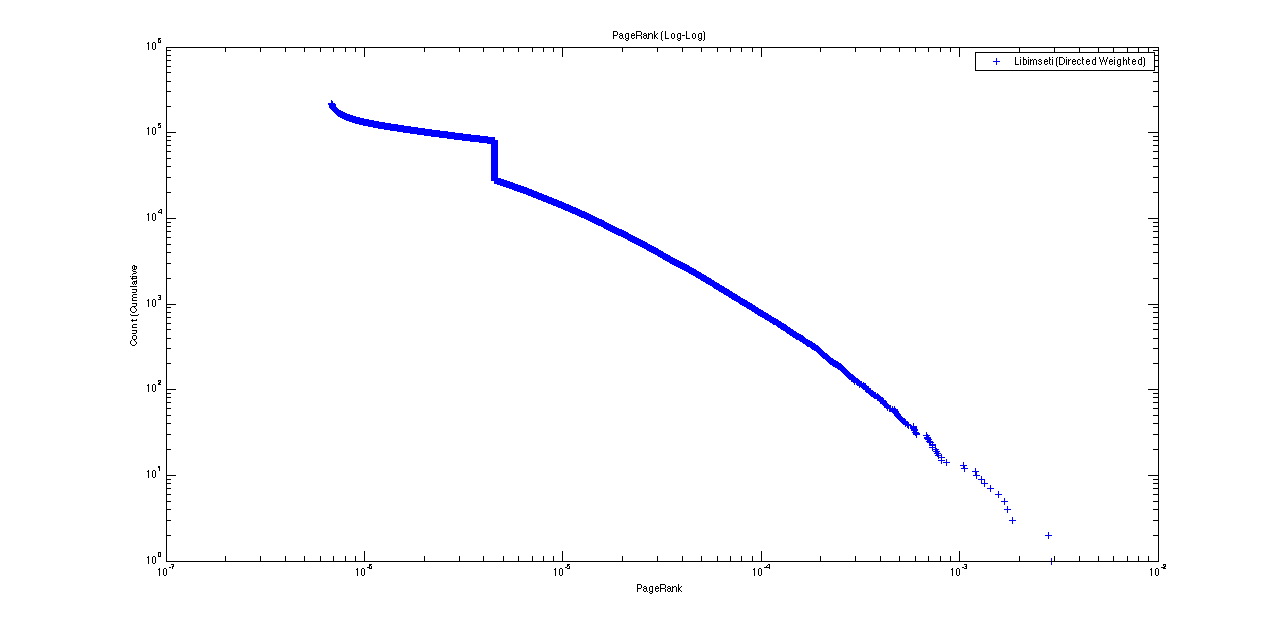
\includegraphics[width=\textwidth]{FIG/pr.png}
            \caption{PageRank Distribution}
            \label{fig:dw-pr2}
    \end{subfigure}
    \caption{PageRank vs Weighted PageRank}
        \label{fig:results8-2}
\end{figure}